% =====================================================================
% Morphological Efficiency in Multilingual Language Models
% Submission to Natural Language Processing (Cambridge University Press)
%
% Typeset in the journal's own cup-journal.cls (journal=nlp).
% Requires `biber` on PATH to resolve citations (biblatex-chicago backend).
% =====================================================================

\documentclass[
  journal=nlp,
  manuscript=article-type,
  year=2026,
  volume=1,
]{cup-journal}

% -- Packages -----------------------------------------------------------
\usepackage{amsmath, amssymb}
\usepackage[nopatch]{microtype}
\usepackage{booktabs}
\usepackage{graphicx}
\usepackage{xcolor}
\usepackage{placeins}        % \FloatBarrier to pin floats inside subsections
% Visible draft placeholder for results still computing on the GPU box.
\newcommand{\ph}[1]{\textcolor{red}{\textbf{[#1]}}}

% Arabic and Mandarin script support. NOTE: this class force-loads biblatex
% during \documentclass processing, before this preamble runs, so polyglossia
% (which must load *before* biblatex) cannot be used here. The `bidi` package
% was tried as a lower-level alternative but was found to globally break the
% class's title-block generation (logo, article-type banner, citation line,
% and affiliation block all silently disappear once bidi is loaded -- traced
% and confirmed via isolated testing). Since our Arabic use is short inline
% words/phrases, not full right-to-left paragraph flow, XeTeX's native
% Script=Arabic font shaping (via fontspec alone) already produces correctly
% joined, correctly ordered glyphs without needing bidi's paragraph-level
% reordering machinery at all.
\usepackage{fontspec}
\newfontfamily\arabicfont[Script=Arabic]{Amiri}
\IfFontExistsTF{SimSun}
  {\newfontfamily\cjkfont{SimSun}[Script=CJK]}
  {\newfontfamily\cjkfont{Noto Serif CJK SC}[Script=CJK]}
\newcommand{\ar}[1]{{\arabicfont #1}}
\newcommand{\zh}[1]{{\cjkfont #1}}
% -----------------------------------------------------------------------

% Figure path
\graphicspath{{../figures/}}

\title{Does Teaching a Language Model Grammar in Advance Make It Cheaper to Build?}

\author{Sameh AbuRadi}
\affiliation{CODE University of Applied Sciences, Berlin\\Supervised by Prof.\ Dr.\ Fabian Geier}
\email[Sameh AbuRadi]{Sameh.AbuRadi@CODE.Berlin}

% Append ORCID after the email in the corresponding-author footnote,
% rather than inside \email{} itself: the class renders that argument
% through \url{}, which cannot carry the extra ", ORCID: ..." text.
\makeatletter
\renewcommand*\cup@contact@details{%
  { \emailsymbol{}Corresponding author. Email: \cup@email@list, ORCID: \url{https://orcid.org/0009-0008-0716-7598}}%
  \cup@number@list
}
\makeatother

\addbibresource{references.bib}

\keywords{grammar-aware tokenisation, morphological typology, transformer scaling laws, linguistic typology, information theory in NLP, computational linguistics, AI and ML economics}

\begin{document}

% -- Abstract -----------------------------------------------------------
\begin{abstract}
Transformer scaling laws (\emph{the empirical curves that predict how a language model's performance grows with its parameter count and the amount of text it is trained on}) are seemingly fitted on analytic-leaning languages such as English and Mandarin, whose words carry little grammatical marking on their written surface. This could genuinely be due to the fact that the AI market is dominated by China and Anglophone regions of the world at the time of writing. This paper asks whether languages at the opposite end of the typological spectrum, whose words inflect richly and write that inflection out in full, can turn their grammatical structure into a measurable computational efficiency factor.

The mechanism we study is \emph{grammar-aware tokenisation}. Instead of chopping text into frequent character fragments by statistics alone (\emph{byte-pair encoding, or BPE for short, which never consults grammar}), we hand the model a grammatical analysis of each word: its part of speech and the bundle of inflectional features it carries (\emph{tense, person, gender, number, case, and so on}). This analysis enters the network as a feature embedding summed with the ordinary token embedding at the input layer. Arabic's templatic nature means that part of that contextual information is stored deeper than the surface, and accordingly it has two further streams exposing the consonantal root and the \emph{wazn} pattern, more on that later. The hypothesis, designed to be tested rather than assumed, is that exposing the morphological structure of our test languages rebates part of their transformers' parameter budgets, and that the rebate scales with how much grammar the writing system already makes visible: a language whose grammar indicates lower morphological information density should gain little; one that indicates more should gain more.

We try to make this precise through a single quantity, $\rho(L) \cdot H(L)$, where $H(L)$ is the Shannon entropy of the grammatical features a word form carries (\emph{a bit-valued measure of how much grammar one word packs}) and $\rho(L)$ is the share of that information legible from the written word itself, without lexical lookup. A rule-based grammar engine computes both before any model is trained, so the cross-linguistic ordering is registered in advance: $\rho \cdot H$ ranks the four languages Mandarin $<$ English $<$ Turkish $<$ Arabic, with values $0.16$, $1.07$, $2.98$, and $3.47$ on the four-language corpora. The same ordering is already visible in the raw inventories the engine produces: across the three inflecting languages the number of distinct grammatical feature bundles attested follows the same rank (\emph{roughly $21$ for English, $469$ for Turkish, and over $1{,}400$ for Arabic}), so the ranking is legible before entropy or surface-recoverability is computed.

The study trains four matched pairs of transformers, a baseline and a grammar-aware model for each of Mandarin, English, Turkish, and Arabic, four languages chosen to span the typological spectrum from isolating through analytic and agglutinative to templatic. Each model holds roughly $3.2 \times 10^7$ parameters in the transformer the two regimes share and is trained on about $6.4 \times 10^8$ tokens (\emph{close to twenty per parameter, the compute-optimal ratio}) drawn from some one billion tokens of mixed encyclopaedic and web-crawl text, five million sentences per language. Because the baseline and grammar-aware tokenisers cut the same text into different numbers of pieces, a per-token loss is not comparable between them; we therefore report bits per character, which scores the cost of the text itself.

Mandarin, the isolating control, behaves as predicted: its baseline and grammar-aware models finish within $0.004$ bits per character of each other, the near-null a language that writes almost no grammar on its surface should show. English, the analytic case, shows no rebate either at this scale, its grammar-aware model finishing $0.036$ bits per character \emph{worse} than baseline. Turkish, the agglutinative case where the hypothesis predicts a clear rebate, also shows none at this scale: its grammar-aware model finishes $0.017$ bits per character worse than baseline. Arabic, the templatic case, is the exception: its grammar-aware model finishes $0.0192 \pm 0.0023$ bits per character \emph{better} than baseline (\emph{mean over four seeds}), the only positive rebate of the four. The pattern that emerges is narrower than the framework's $\rho \cdot H$ ordering. The rebate appears only for the language whose grammar is least legible from the written surface (Arabic, the lowest $\rho$, whose root-and-pattern system hides structure off the surface), and is absent wherever a compute-optimal model can read the grammar off the text for itself (Mandarin, English, Turkish). One caveat could temper the Arabic result: its grammar-aware model also carries the most additional embedding parameters (the root and \emph{wazn} streams raise its parameter count by roughly half). A parameter-matched ablation settles it: scrambling the content of those two streams while holding their size fixed makes the model finish \emph{below} its own baseline, and the real streams beat the scrambled ones by $0.043$ bits per character, so the gain is attributable to templatic structure rather than to added capacity.

A smaller three-language pilot first surfaced an ordering by $\rho \cdot H$ and motivated this study; the four-language test overturns it. At compute-optimal, transformer-matched scale (\emph{the grammar-aware models carry more total parameters, which only makes the null results more conservative}), the rebate vanishes for the three languages whose grammar is surface-legible, Turkish included, the agglutinative case the pilot most favoured, because a model with enough data learns their grammar from the text itself, making an explicit morphological analysis redundant. It survives only for Arabic, whose templatic morphology hides grammar off the surface, and a shuffle-control ablation indicates that survival is structural rather than a parameter artefact. Where the lever exists at all, it appears to track the grammar a language hides off the surface rather than the recoverable $\rho \cdot H$ the framework first proposed; with a single positive language, this is a conjecture for a larger study, not a law we establish. The practical promise, on-device modelling of grammar-rich languages at parameter counts English does not reach (\emph{a frontier that compact edge models such as Google's Gemma~4 E4B, a 2026 on-device model that appeared while this research was underway and uses per-layer embeddings to reach roughly four billion effective parameters while still fitting on a phone, are already approaching}), therefore narrows to the templatic case, where it is strongest and where current pipelines serve worst.
\end{abstract}


% -- Body ---------------------------------------------------------------
\section{Introduction}
\label{sec:intro}

\paragraph{Plain-language summary.} A language model must learn the grammar of its language
from examples alone, spending part of its capacity on that. We test a simple alternative:
give the model the grammatical analysis of each word directly. Across four languages chosen
to span very different grammatical styles, the shortcut pays off in exactly one case,
Arabic, and for a clear reason. Arabic keeps much of its grammar off the page, in the vowel
pattern woven through a word's consonants that everyday writing leaves out, so a model
reading raw text cannot recover it however much it reads; handing that hidden structure over
directly saves it real work. Languages that write their grammar out in full let the model
learn it unaided, and the shortcut earns nothing. The effect is small but consistent: it
repeats across four independent training runs, and a control that scrambles the grammatical
information, keeping everything else identical, removes it entirely, showing that it is the
\emph{structure} that helps and not the extra machinery.

Two observations about the current state of language modelling sit in quiet tension. The first is that the abilities we associate with reasoning (multi-step arithmetic, long-context inference, writing working code) appear, by a range of measurements, only once standard English-centric transformers exceed $10^{10}$ parameters \citep{wei2022}. The second is that the parameter counts a consumer device can actually hold (smartphones, laptops with integrated GPUs, embedded devices) sit well below this threshold, even after aggressive compression to 4 bits per weight or lower (roughly $5 \times 10^{8}$ to $2 \times 10^{9}$ parameters on current mobile chips). The gap between these two figures is why reasoning-capable language models live, at present, as cloud services rather than on the device in the user's hand.\footnote{This on-device ceiling has recently begun to rise. Google's Gemma project, in particular, uses per-layer embeddings to expose a larger effective parameter count than a device must hold in high-speed memory at once: the Gemma~4 E4B model \citep{gemma4} reaches roughly four billion effective parameters while remaining phone-deployable. Such systems are too recent for their capability-per-parameter to be assessed with confidence, and we note them as an indication of direction rather than as a settled datum.}

Most treatments frame this gap as a problem of scale, to be closed by compression, quantisation, distillation, or architectural cleverness. What that framing leaves unexamined is that the figures on both sides are fit to English: transformer scaling laws \citep{kaplan2020, hoffmann2022} are calibrated on predominantly English corpora, and the benchmarks tracking the onset of reasoning inherit English as their default medium. Whether the same parameter thresholds hold for languages whose grammar is organised quite differently, packing more information into each word form or writing it more legibly on the surface, is not a settled question; for the most part it is not even an asked one.

Responses to the gap between edge and reasoning fall along three axes the field rarely names in one breath. The first, and most heavily funded, is \emph{brute-force hardware scaling}: larger datacentre GPUs (Nvidia's H- and B-series), more high-bandwidth memory, more interconnect, more electrical power, on the bet that capability per dollar will keep bending favourably with scale. The second, more speculative, is \emph{substrate redefinition}: companies such as Extropic \citep{extropic2024} are building \emph{thermodynamic sampling units}, chips that are inherently probabilistic, arguing that modern AI inference is at heart a sampling workload whose deterministic emulation on transistor silicon is physically wasteful. The third, which this paper develops, sits one layer above both. Rather than adding hardware or rewriting its physics, it aligns the tokenisation layer to the grammatical structure of the language being modelled, freeing up compute on the existing GPU substrate that is currently spent on learning grammar from distributional statistics. The three routes are not mutually exclusive, but they cut the cost problem very differently. Nvidia spends more energy to train the same languages faster; Extropic proposes spending much less energy under a different computational paradigm; grammar-aware tokenisation spends nothing extra and recovers compute by changing what the model has to learn in the first place.

This paper develops the possibility that the parameter threshold for a given capability depends, in a measurable way, on the language. More precisely: a transformer trained under a tokenisation that respects a language's morphological structure, where \emph{grammatical feature bundles} (the parsed grammatical analysis of each word) are handed to the model as explicit categorical inputs rather than reconstructed from the co-occurrence of byte-pair fragments, is spared a portion of the parameter budget its byte-pair counterpart must spend on rebuilding that structure from scratch.

A \emph{grammatical feature bundle}, in the sense used throughout this paper, is the complete set of grammatical category and value pairs that a single word form realises at once. Following the paper's typological order: the Mandarin \zh{书} (\emph{sh\=u}, ``book'') carries only $\{\text{NOUN}\}$, its number and definiteness left to context and particles rather than marked on the word; the English \emph{researchers} adds one feature, $\{\text{NOUN}, \text{number}=\text{plural}\}$; the Turkish \emph{evlerinizden} stacks several, $\{\text{NOUN}, \text{number}=\text{plural}, \text{possessor}=\text{2-person plural}, \text{case}=\text{ablative}\}$; and the Arabic \ar{اسْتَخْدَمَ} (\emph{istakhdama}, ``he used'') carries $\{\text{VERB}, \text{form}=\text{X}\}$. That last value rewards a closer look, because it is where Arabic departs from the other three languages. An Arabic word is built along two orthogonal axes at once: a consonantal root that fixes the semantic field (here \ar{خ-د-م}, \emph{kh-d-m}, the serving-related meaning) and a pattern, or \emph{wazn}, woven through it that fixes the grammatical and derivational meaning. \emph{Form~X} (\ar{اسْتَفْعَل}) is the pattern of seeking, requesting, or considering-to-be, so \emph{istakhdama} reads literally as ``he sought service'' before lexicalising to ``he used''. The flat tag $\text{form}=\text{X}$ therefore stands in for a whole second dimension of structure: grammatical information interleaved through the consonants rather than appended to them. This root-and-pattern two-dimensionality, together with neuroimaging evidence that it places distinctive demands on the semantic language network of native Arabic speakers \citep{wei2023native}, is among the phenomena that motivated this study. Bundles are the unit of grammatical information the framework quantifies. They are what a morphology-aware tokeniser encodes outright, what a byte-pair tokeniser leaves the model to recover from distributional statistics, and what the two quantities introduced next, $H(L)$ and $\rho(L)$, respectively measure the Shannon entropy and the structural recoverability of.

The rebate is set by two quantities a grammar engine computes before any training run, and which \S\ref{sec:framework} defines formally: the entropy $H(L)$ of a word's grammatical features, and the fraction $\rho(L)$ of them legible from the written surface. The framework predicts that their product $\rho(L) \cdot H(L)$ orders the parameter rebate across languages, and, under a stated linearity assumption, that a single cross-lingual constant $\alpha$ turns the product into a quantitative prediction.

The core of this paper is a four-language experiment. For each of Mandarin, English, Turkish, and Arabic, languages chosen to span the typological spectrum from isolating through analytic and agglutinative to templatic, we train a baseline and a grammar-aware transformer identical in every respect but the tokeniser. The two share an identical transformer; the grammar-aware model carries extra embedding parameters for its additional streams (\S\ref{sec:results-design}), so the pair is matched in the transformer, not in total parameters. Both train at a compute-optimal token budget and are compared in bits per character, a measure independent of how each tokeniser cuts the text. The grammar engine fixes the prediction before any model trains: $\rho(L) \cdot H(L)$ ranks the four languages Mandarin $<$ English $<$ Turkish $<$ Arabic. If grammar is a capacity lever, the rebate should follow that order, smallest for the isolating language whose grammar barely reaches the written surface and largest for the templatic language that packs the most grammatical information into each word.

This four-language test grew out of a smaller pilot. An earlier, budget-limited experiment on three languages (English, Arabic, and Turkish) at roughly two million parameters first showed the ordinal effect, the test-loss reduction under morphology-aligned tokenisation falling in the same rank order as $\rho \cdot H$. It also surfaced a magnitude puzzle, an apparent acceleration of the per-bit rebate with $\rho \cdot H$ that we named the \textbf{Agglutinative Compounding Effect}, and a companion observation for Arabic, the \textbf{Templatic Lexical Surplus}, in which exposing the consonantal root as its own input stream bought a further rebate beyond surface morphology. The pilot trained far below the compute-optimal budget and on only three points, so it could not separate a genuine property of grammar-aware modelling from an artefact of English-centric scaling laws applied out of range. The four-language experiment is built to settle what the pilot could not.

The paper makes four contributions. The first is a framework in which a language's grammatical structure maps to a quantitative prediction about transformer parameter requirements, with inputs ($H(L)$ and $\rho(L)$) computable from a grammar engine before any training begins. The second is the four-language, parameter-matched, compute-optimal test of that prediction, the first to place the comparison inside the regime where the scaling laws were fitted and to score it in tokeniser-neutral bits per character. The third is the engine-derived ordering, $\rho \cdot H$ ranking Mandarin $<$ English $<$ Turkish $<$ Arabic, registered in advance as the prediction the experiment tests. The fourth is the pilot and its two named observations, the \textbf{Agglutinative Compounding Effect} and the \textbf{Templatic Lexical Surplus}, which motivated the study and which the four-language results will either confirm or dissolve.

The Templatic Lexical Surplus deserves a word here, because it is what the root-and-pattern two-dimensionality of \S\ref{sec:intro} points to in practice. Arabic stores much of its grammatical information off the written surface, behind the interleaving of root and pattern, so a surface-only $\rho(L)$ under-prices it. The pilot found that giving the model the consonantal root as its own input stream recovered a measurable rebate beyond surface morphology, one that held even where the surface-level advantage faded. The four-language experiment carries this forward: Arabic is modelled with explicit root and \emph{wazn} streams, and \S\ref{sec:results} reports whether the surplus survives at compute-optimal scale. The paper takes no side in advance between the two readings of the pilot's effect; the four-language results are what decide between them.

Edge-hostable reasoning, reasoning-capable models that fit inside smartphone-class budgets, is the motivation for the question, not a claimed result. It is a conditional: \emph{if} grammar-aware tokenisation is a genuine capacity lever rather than an artefact of the pilot's under-trained regime, then it becomes a plausible near-term prospect for grammatically rich languages, at parameter counts English does not currently reach. Whether that conditional holds is what the four-language experiment is designed to answer.

The remainder of the paper is organised as follows. \S\ref{sec:related} places the work inside five neighbourhoods of prior art: morphological typology, tokenisation in NLP, transformer scaling laws, the framing of capability emergence, and the Green AI, linguistic equity, and edge ML literature on cost. \S\ref{sec:framework} develops the framework formally. \S\ref{sec:cases} walks through Mandarin, English, Turkish, and Arabic morphology, with the grammar-engine decompositions that supply the framework's inputs. \S\ref{sec:results} reports the four-language experiment, with the pilot that motivated it summarised in brief. \S\ref{sec:discussion} discusses the consequences of each interpretation, together with the limitations that bound confidence in the observation. \S\ref{sec:conclusion} concludes and specifies the discriminating research programme.

\section{Related Work}
\label{sec:related}

The framework developed in \S\ref{sec:framework} sits at the meeting point of five literatures. Each contributes an input or a constraint, and none of them, on its own, asks the question this paper poses.

\subsection{Morphological typology}
\label{sec:related-typology}

Classifying languages by the way they organise grammatical information inside the word form is a century-old project. \citet{greenberg1960} introduced a family of quantitative indices, most prominently the \textbf{Index of Synthesis} (the average number of morphemes per word in a corpus) and the \textbf{Index of Agglutination} (the ratio of clean, agglutinative morpheme boundaries to fused, portmanteau ones). These indices placed analytic, agglutinative, and fusional languages on continuous rather than categorical scales. \citet{comrie1989} and \citet{haspelmath2010} extend this typological work with richer treatments of inflection, derivation, and the interplay between morphology and syntax. Together these works describe how much grammatical information languages encode, and how they encode it. They do not, in general, ask what consequences the encoding has for computational models of the language.

The Structural Synthesis Ceiling introduced in \S\ref{sec:framework-ssc} stands explicitly in this lineage. It differs from Greenberg's Index of Synthesis in being a structural upper bound rather than a corpus average: the maximum grammatical information a word form can express in principle, rather than the average of what it does express in a given sample. We need this distinction because the framework's prediction target is the information a tokeniser can \emph{pre-encode}, which is bounded by what the morphology permits rather than by what a particular text happens to use.

\subsection{Morphology-aware tokenisation in NLP}
\label{sec:related-tokenisation}

Byte-pair encoding and its variants \citep{sennrich2016, kudo2018} have become the default way of splitting text into modelling units in large language modelling, valued for their simplicity, robustness, and the fact that they make no linguistic commitments. That last property is also their limitation. BPE fragments are simply the output of a frequency-driven compression procedure, so morphemes, the actual carriers of grammatical meaning, appear in the resulting vocabulary only by accident.

A recurring strand of work in multilingual NLP has tried to bring tokenisation closer to morphology, especially for agglutinative and templatic languages, where BPE's purely statistical splits do markedly worse than a proper morphological analysis. Representative examples include compositional, morphology-aware input representations for Turkish neural machine translation \citep{ataman2018}, and evidence that unigram-LM tokenisation recovers subword units that align more closely with morpheme boundaries than BPE across typologically diverse languages \citep{bostrom2020}. These works show that morphology-aware tokenisation can improve internal measures such as perplexity and vocabulary coverage, and some downstream tasks, for specific languages. Their framing, however, is almost always empirical: \emph{does this tokeniser work better for this language on this task?} The framework of \S\ref{sec:framework} asks a structurally different question, \emph{how much grammatical information does this language allow a tokeniser to pre-encode, and what does that imply for the number of parameters a transformer needs?}, and it answers using quantities that can be computed without running any training experiment.

A parallel and largely separate strand of work addresses Arabic, whose root-and-pattern morphology resists statistical segmentation in particular ways. The Buckwalter analyser \citep{buckwalter2004} pairs a stem dictionary with prefix and suffix concatenation tables, and remains the cornerstone of computational Arabic morphology. The MADA system of \citet{habash2005mada}, later extended in \citet{habash2009mada}, treats morphological analysis as a disambiguation problem over the analyser's candidate parses, selecting a fully specified morphological tag from context. MADAMIRA \citep{pasha2014madamira} consolidated this line of work into a practical tagger combining MADA with the AMIRA tokeniser. These systems are descriptive: given a surface word, they return its analysis. The framework of \S\ref{sec:framework} uses morphological analysis in the opposite direction, as a structured input stream to a transformer's tokeniser rather than as an end product, and asks what the analyser's output implies for parameter cost.

Chinese has its own small but established literature on bringing sub-character structure into the input representation. \citet{sun2014radical} introduced radicals as an auxiliary embedding signal alongside character embeddings; \citet{shi2015radical} pushed this further with a dedicated radical embedding scheme that decomposes each character into its constituent radicals. \citet{cao2018cw2vec} took the decomposition one level deeper, using stroke n-grams over the canonical writing order. These approaches treat sub-character information as the principal or sole representational unit, replacing or augmenting the character embedding. The framework of \S\ref{sec:framework} differs in that the radical-class layer is added as a structured input stream alongside character tokenisation, not in place of it, and the question asked of that layer is again structural: how much grammatical and semantic information does the radical inventory permit a tokeniser to pre-encode, independent of any particular training run.

\subsection{Transformer scaling laws}
\label{sec:related-scaling}

\citet{kaplan2020} described the relationship between a transformer's test loss and its parameter count, training tokens, and compute budget as a set of power laws with specific empirical exponents. \citet{hoffmann2022}, best known for the Chinchilla compute-optimal result, refined the relationship into the form $\mathcal{L}(N, D) = E + A \cdot N^{-\alpha_N} + B \cdot D^{-\alpha_D}$ and identified the compute-optimal ratio of roughly twenty training tokens per parameter. More recent work has extended these laws into questions of how much information each parameter can store. \citet{allenzhu2024}, in a study of the upper limits of transformer knowledge storage, report a saturation coefficient of about two bits per parameter, stable across architectures and training configurations. Equation~\ref{eq:Cexplicit} of \S\ref{sec:framework} uses this coefficient as its working value of $\kappa$.

This literature provides the quantitative machinery that \S\ref{sec:results} uses to relate test loss to parameter count, and it underlies the finding, developed in \S\ref{sec:discussion-ace}, that the pilot's apparent rebate was an artefact of training below the compute-optimal ratio. The scaling laws are fitted on predominantly English corpora, and how well they carry over to morphologically distant languages is an open question the four-language result speaks to directly.

\subsection{Emergence and capability-scale curves}
\label{sec:related-emergence}

How new capabilities appear as transformers grow is an actively contested question. \citet{wei2022} reported that certain abilities, chain-of-thought reasoning in particular, appear sharply once parameter counts exceed specific thresholds, typically in the $10^{10}$ to $10^{11}$ range for English models. \citet{schaeffer2023} replied that much of what is reported as emergence is a side-effect of all-or-nothing scoring metrics, such as exact-match or threshold-based accuracy. Under smoother, continuous metrics, the curves relating capability to model scale are typically gentle, sigmoidal. The framework of \S\ref{sec:framework} stays neutral between these readings. Equation~\ref{eq:curveshift} predicts that morphology-aligned tokenisation shifts the capability-versus-scale curve to the left, and whether that curve is sharp or smooth does not change the form of the prediction.

\subsection{Green AI, linguistic equity, and edge ML}
\label{sec:related-economics}

A fifth literature treats the cost of machine learning as an economic, environmental, and equity question rather than a purely technical one. \citet{strubell2019} measured the energy use and carbon footprint of training large language models. \citet{schwartz2020} proposed Green~AI as a research orientation that takes efficiency seriously as a first-class goal rather than as an afterthought. \citet{bender2021}, in the Stochastic Parrots paper, raised concerns about the linguistic scope of the models the field is building, noting that the cost and data demands of the dominant paradigm systematically disadvantage languages outside the high-resource, English-centric mainstream. \citet{ahia2023} measured the per-language compute gap in multilingual NLP directly.

The framework of \S\ref{sec:framework} adds to these concerns a specific quantitative route by which language structure enters the cost calculation. Whether grammatically rich languages are \emph{more} expensive to model, the common assumption, based on lower data availability and higher surface diversity, or \emph{less} expensive, is a question the framework makes tractable; \S\ref{sec:results} answers it for four languages, finding the saving real only for the templatic case whose grammar is hidden off the surface (\S\ref{sec:discussion-tls}). The answer bears directly on how research compute, data collection effort, and model-sharing agreements should be allocated across the world's languages.

\section{Framework}
\label{sec:framework}

This section develops a framework that predicts, from a language's grammar alone, how much grammar-aware tokenisation lowers the parameter count a transformer needs to reach a fixed capability threshold. The framework is built in six moves. \S\ref{sec:framework-ssc} defines the \textbf{Structural Synthesis Ceiling}, a structural upper bound on the grammatical information a single word form can carry, and sets it apart from Joseph Greenberg's corpus-averaged Index of Synthesis. \S\ref{sec:framework-H} gives the information-theoretic quantity $H(L)$, the grammatical Shannon entropy per word form. \S\ref{sec:framework-rho} introduces the \textbf{structural recoverability coefficient} $\rho(L)$, which captures how much of $H(L)$ is recoverable by a regular surface-only parser. \S\ref{sec:framework-A1} states the assumption (A1) that ties grammatical information to model capacity, and names the \emph{implicit grammar cost} a BPE-tokenised transformer must pay. \S\ref{sec:framework-engine} describes the per-language engine architecture (a morphology layer plus a grammar layer, together with the categorical input streams they emit) through which $B(L)$ becomes a concrete embedding table. \S\ref{sec:framework-rebate} combines these into a closed-form prediction for the \textbf{parameter rebate} $\Delta N(L)$ that morphology-aligned tokenisation delivers relative to BPE, and spells out the corresponding \textbf{capability-vs-scale curve shift}. The empirical status of this prediction is the subject of \S\ref{sec:results}.

\subsection{The Structural Synthesis Ceiling}
\label{sec:framework-ssc}

Consider a language $L$ whose morphology realises grammatical features on word forms through any combination of inflection, derivation, affixation, and non-concatenative processes. For each grammatical category $C$ encoded in $L$'s morphology (tense, aspect, mood, person, number, gender, case, definiteness, possession, polarity, and so on, the inventory varying from language to language), let $V(C)$ be the set of values that category admits. Let $B(L)$ be the set of distinct grammatical feature bundles that $L$'s morphology can realise simultaneously on a single word form, once syncretism, defectiveness, and paradigm gaps have been taken into account. $B(L)$ is, in effect, the realised subset of the Cartesian product $\prod_C V(C)$, the structural ``address space'' of a word form in $L$.

We define the \textbf{Structural Synthesis Ceiling} (SSC) of $L$ as the cardinality of $B(L)$, and its logarithm in bits:

\begin{equation}
\mathrm{SSC}(L) = |B(L)|, \qquad H_{\max}(L) = \log_2 |B(L)|.
\label{eq:ssc}
\end{equation}

$H_{\max}(L)$ is the maximum grammatical information, in bits, that a single word form can carry, independent of any corpus, tokeniser, or training run. It can be read off a language's grammar description alone, and in our implementation it is enumerated directly from the feature-bundle registry of each language's grammar engine.

SSC sits within a lineage of typological indices, but differs from its best-known predecessor. \citet{greenberg1960} defined the \textbf{Index of Synthesis} as the average number of morphemes per word, computed over a corpus. The Index of Synthesis is a \emph{descriptive} typological measure, telling us how many morphemes are strung together in a representative sample of text. SSC is instead a \emph{structural upper bound}, telling us how many distinct grammatical specifications the morphology can in principle express on a single word, regardless of how often each is realised in practice. The Index of Synthesis is empirical and averaged; SSC is combinatorial and peaked. For our purposes, predicting how much grammatical information a tokeniser can pre-encode, the structural ceiling is the relevant quantity.

For the four languages this paper tests, the structural ceiling $|B(L)|$ spans more than two orders of magnitude, tracking the morphological typology from isolating to templatic (Table~\ref{tab:framework-inputs}). Mandarin marks almost no grammar on the word form itself; the structural signal it carries lives not in inflection but in the Kangxi radical layer (\S\ref{sec:framework-engine}). English, analytic, has the smallest inflectional ceiling of the three inflecting languages, $|B(L)| = 89$ ($H_{\max} \approx 6.48$ bits). Turkish, agglutinative, stacks suffixes in a strict slot order into $|B(L)| = 4{,}382$ realisable bundles ($H_{\max} \approx 12.10$ bits). Arabic, a root-and-pattern templatic language whose grammar arises from interleaving consonantal roots (mostly triliteral, with a smaller class of quadriliteral roots and a handful of longer ones) with vowel patterns (\ar{أَوْزَان}, \emph{awz\=an}), reaches $|B(L)| = 9{,}579$ ($H_{\max} \approx 13.23$ bits), roughly twice Turkish's structural space and with a comparable ceiling, the two synthetic systems approaching each other from opposite mechanisms: Turkish by combinatorial slot-stacking, Arabic by templatic interleaving.

\begin{table}[hbt!]
\centering
\begin{tabular}{llrrrrrr}
\toprule
Language & Type & $|B(L)|$ & obs. & $H_{\max}$ & $H(L)$ & $\rho(L)$ & $\rho \cdot H$ \\
\midrule
Mandarin & isolating     & $547$   & $131$   & $9.10$  & $6.28$ & $0.025$ & $0.16$ \\
English  & analytic      & $89$    & $21$    & $6.48$  & $1.30$ & $0.822$ & $1.07$ \\
Turkish  & agglutinative & $4{,}382$ & $469$ & $12.10$ & $4.01$ & $0.744$ & $2.98$ \\
Arabic   & templatic     & $9{,}579$ & $1{,}450$ & $13.23$ & $6.51$ & $0.534$ & $3.47$ \\
\bottomrule
\end{tabular}
\caption{Engine-derived inputs to the framework, computed from the four-language corpora before any model is trained. $|B(L)|$ is the \emph{structural} bundle-space ceiling: the distinct grammatical feature bundles the morphology can realise, enumerated from the grammar engine and independent of any corpus. The \emph{obs.}\ column is the number of distinct bundles actually attested in the full corpus, which is smaller and corpus-dependent. $H_{\max} = \log_2 |B(L)|$; $H(L)$ is the corpus-weighted grammatical entropy (\S\ref{sec:framework-H}) and $\rho(L)$ the fraction of it recoverable from the written surface (\S\ref{sec:framework-rho}). Mandarin's $H(L)$ reflects character-and-radical serialisation rather than inflection (\S\ref{sec:framework-H}). The framework's prediction is that the parameter rebate is ordered by the final column: Mandarin $<$ English $<$ Turkish $<$ Arabic.}
\label{tab:framework-inputs}
\end{table}
\FloatBarrier

A note on terminology. $|B(L)|$ is the \emph{structural} ceiling just defined, a property of the grammar; the \emph{obs.}\ column of Table~\ref{tab:framework-inputs} is the smaller, corpus-dependent count of bundles actually attested, which grows with corpus size (Arabic's $9{,}579$ realisable bundles surface as $1{,}450$, Turkish's $4{,}382$ as $469$). It is these observed counts, not the ceiling, that feed the distribution-weighted $H(L)$ of \S\ref{sec:framework-H}, which is therefore stable as more text is seen; the canonical structural quantities remain $|B(L)|$ and $H_{\max}(L)$.

\subsection{Grammatical information content $H(L)$}
\label{sec:framework-H}

$H_{\max}(L)$ is only an upper bound. The grammatical information actually carried by an average word form depends on how bundles are distributed in naturally occurring text. Let $p(b)$ denote the empirical probability, over a corpus of $L$, that a given word form carries feature bundle $b \in B(L)$. The \textbf{grammatical information content} of $L$, in bits per word form, is the Shannon entropy over this distribution:

\begin{equation}
H(L) = -\sum_{b \in B(L)} p(b) \, \log_2 p(b).
\label{eq:H}
\end{equation}

$H(L) \le H_{\max}(L)$, with equality only when every bundle is equiprobable. In practice the realised distribution is highly skewed. A handful of common bundles (third-person singular present in English, nominative singular in Turkish, Form~I active perfective in Arabic) dominate, and $H(L)$ falls well below the ceiling (Table~\ref{tab:framework-inputs}). Mandarin's figure ($6.28$ bits) is anomalous and must be read with care: it reflects the breadth of the engine's character-and-radical bundle serialisation rather than inflectional richness, since Mandarin marks almost no inflection on the word. What matters for the framework is that Mandarin's surface recoverability $\rho$, and therefore its $\rho \cdot H$, comes out by far the lowest of the four (\S\ref{sec:framework-rho}).

For the three inflecting languages, the ordering of $H(L)$, English $<$ Turkish $<$ Arabic, tracks their grammatical density directly. The product $\rho \cdot H$ that the framework actually predicts on is developed next.

\subsection{Structural recoverability $\rho(L)$}
\label{sec:framework-rho}

$H(L)$ measures the grammatical information a word form carries. It does not measure how much of that information is accessible to a surface-only parser, that is, a parser that sees the word's surface string and nothing else, with no access to a lexicon and no context. The distinction matters because tokenisers, whether BPE or morphology-aligned, work on surface forms.

We capture this distinction with a single coefficient. Let $s \in \Sigma$ range over surface forms and $b \in B(L)$ over feature bundles. The \textbf{conditional entropy of the bundle given the surface form} is:

\begin{equation}
H(b \mid s) = \sum_{\sigma \in \Sigma} p(\sigma) \cdot H(b \mid s = \sigma),
\label{eq:Hcond}
\end{equation}

where $H(b \mid s = \sigma)$ is the Shannon entropy of the bundle distribution conditional on the specific surface form $\sigma$, estimated from corpus-observed $(s, b)$ pairs. We define the \textbf{structural recoverability coefficient} of $L$ as:

\begin{equation}
\rho(L) = 1 - \frac{H(b \mid s)}{H(L)}.
\label{eq:rho}
\end{equation}

Equation~\ref{eq:rho} reads off directly. $H(b \mid s)$ measures the grammatical uncertainty that remains once the surface form has been observed. When the morphology is one-to-one with its surface realisation, with each bundle corresponding to a unique surface string as in an idealised agglutinative language, $H(b \mid s) = 0$ and $\rho = 1$. When the surface form carries no information at all about the bundle, the degenerate case of complete ambiguity, $H(b \mid s) = H(L)$ and $\rho = 0$. Real languages fall in between.

Two technical points deserve mention. First, the conditional entropy~\ref{eq:Hcond} is conditioned on the surface string itself, rather than on a ``surface signature'' produced by stripping the lexical content. For concatenative morphologies such as English and Turkish, a lemma-stripped signature differs from the full surface only in lexical root identity, which in principle carries no grammatical information. For templatic morphologies such as Arabic, the grammar engine's explicit \texttt{template} field, a categorical label naming the morphological pattern (for instance \texttt{VERB\_TRILATERAL\_BARE} or \texttt{NOM\_DERIVED}), plays this role directly. Second, $\rho(L)$ is a property of the language's grammar together with its corpus distribution, not of any particular tokeniser. Both BPE and morphology-aligned tokenisers, as surface-only systems, are bounded above in the grammatical information they can recover by $H_{\mathrm{eff}}(L) = \rho(L) \cdot H(L)$.

The computed values (Table~\ref{tab:framework-inputs}) reflect the typological character of the four systems. Mandarin sits near zero ($\rho \approx 0.025$): almost none of what the engine serialises as a bundle is recoverable from the bare character string, which is exactly why its $\rho \cdot H$ collapses to $0.16$ despite the inflated raw $H$. English and Turkish, both fundamentally concatenative, expose most of their grammatical structure on the surface ($\rho \approx 0.82$ and $0.74$). Arabic's templatic fusion hides close to half of the grammatical signal ($\rho \approx 0.53$) behind ambiguities that lexical context or full analysis would be required to resolve. The resulting product $\rho \cdot H$ is the engine-derived prediction the experiment tests, ordered Mandarin $<$ English $<$ Turkish $<$ Arabic. The absolute values are signature-proxy estimates; a more refined estimator, for instance the mutual information between surface suffix $n$-grams and bundles, is left to follow-up work.

\subsection{Implicit grammar cost and Assumption A1}
\label{sec:framework-A1}

A transformer trained on byte-pair tokens receives no structural information about morphology at its input. Grammatical structure (which bundles go with which lexical material, which inflections follow which roots, which surface patterns realise which feature combinations) has to be learned from co-occurrence statistics in the training data. That learning consumes model capacity.

Let $C_{\mathrm{implicit}}(L)$ denote the model capacity, in bits, that a BPE-trained transformer must allocate to reconstructing $H_{\mathrm{eff}}(L)$ from the distribution, at a capability threshold to be specified. Under morphology-aligned tokenisation, the same grammatical information is instead handed to the model as an explicit categorical input: a bundle-embedding table indexed by $b \in B(L)$, summed into the model's input representation alongside the root embedding. The table the implementation actually builds is sized to the corpus-attested bundles, $B_{\mathrm{obs}}(L) \subseteq B(L)$ (the \emph{obs.}\ column of Table~\ref{tab:framework-inputs}), not the full structural ceiling: a bundle the grammar can in principle realise but that never surfaces in training data earns no row. The capacity cost of the explicit path is just the storage of that table:

\begin{equation}
C_{\mathrm{explicit}}(L) = |B_{\mathrm{obs}}(L)| \cdot d_{\mathrm{embed}} \cdot (\text{bits per weight}).
\label{eq:Cexplicit}
\end{equation}

Even at the largest configuration used here (the Arabic grammar-aware model, whose bundle stream indexes $1{,}450$ observed bundles and whose root and \emph{wazn} streams add a further $7{,}142$ and $185$ entries, at $d_{\mathrm{embed}} = 512$), each individual embedding table is small in absolute terms. For the one- and two-stream languages the categorical tables are a modest fraction of the transformer they feed, and $C_{\mathrm{explicit}}(L)$ is negligible beside $C_{\mathrm{implicit}}(L)$. Arabic is the exception. Its four streams, together with the wider surface vocabulary the grammar-aware regime carries, raise its parameter count materially above its baseline (\S\ref{sec:results-design}), far enough that $C_{\mathrm{explicit}}$ cannot be assumed away. We therefore retain the term in the rebate expression below and neglect it only where it is genuinely small; for the Arabic case we settle the question not by assumption but with a parameter-matched shuffle-control ablation (\S\ref{sec:results-ablation}), which holds these embeddings fixed and randomises only their content.

The harder quantity to pin down is $C_{\mathrm{implicit}}(L)$. A precise derivation from first principles would require a theory of how transformers allocate parameters to distributional pattern-learning, and no such theory exists in tractable form. We therefore promote a functional form to a stated assumption, to be examined empirically in \S\ref{sec:results}.

\paragraph{Assumption A1 (dominant-term linearity).}
The capacity a BPE-trained transformer allocates to implicitly reconstructing grammatical structure is, to first order, linear in the effective grammatical information content $\rho(L) \cdot H(L)$:
\begin{equation}
C_{\mathrm{implicit}}(L) = \alpha \cdot \rho(L) \cdot H(L) + O(\text{lower-order terms}).
\label{eq:A1}
\end{equation}

The coefficient $\alpha$ absorbs factors we take to be approximately constant at fixed architecture, data scale, and tokeniser family: the inefficiency of BPE fragments as morphological units, the effective vocabulary over which the grammatical association has to be learned, and the bits-per-parameter capacity of the underlying transformer \citep{allenzhu2024}. One of these is only approximately language-invariant: BPE fragments a templatic script such as Arabic quite differently from an isolating one such as Mandarin, so $\alpha$ may carry residual cross-language variance, which the pilot's scattered per-language estimates already hint at (\S\ref{sec:results-pilot}).

A1 makes a specific bet, and it is worth naming the bet before testing it. It stakes the rebate on the \emph{recoverable} grammatical information $\rho(L) \cdot H(L)$, reasoning that this is what a BPE model must reconstruct from distributional statistics. The opposite reading is equally available: information legible from the surface is exactly what a model trained on enough data can learn unaided, so the capacity a BPE model genuinely cannot spare may instead track the \emph{unrecoverable} fraction $(1-\rho(L))\,H(L)$, the grammar no quantity of surface text reveals. We commit to the $\rho \cdot H$ form as the pre-registered prediction: it is not a theorem but the hypothesis under test, and \S\ref{sec:results} is built to decide between it and the $(1-\rho)\,H$ alternative it could lose to.

\subsection{Engine architecture: the morphology layer, the grammar layer, and the input streams}
\label{sec:framework-engine}

The previous subsections treated $|B(L)|$, $H(L)$, and $\rho(L)$ as abstract quantities derivable from a language's grammar. They are also concrete outputs of a piece of software, the per-language \emph{morphology engine}, whose architecture we describe here. The engine matters to the framework for two reasons. It is the operational source of the bundle inventory $B(L)$ that anchors Equation~\ref{eq:ssc}, and it determines the shape of the input that the morphology-aligned transformer receives, which in turn fixes what is meant by ``explicit categorical input'' in \S\ref{sec:framework-A1}.

\paragraph{Two layers, one composition.}
Each language is served by a two-layer engine. The lower layer, the \emph{morphology engine}, operates per word. For a given surface form it emits a \texttt{TokenInfo} record containing the surface string, the root or stem, a feature-bundle (part of speech together with the grammatical tags the morphology realises on that word), and a small number of language-specific extras (templatic class for Arabic, radical class for Mandarin, and so on). The upper layer, the \emph{grammar layer}, operates per sentence. It does two things. First, it uses neighbour context to resolve part-of-speech ambiguities that no per-word analyser can settle on its own (the English \emph{run} verb-or-noun question, the Turkish verbal-noun-versus-finite-verb question, the Arabic \ar{مدرسة} school-or-teacher-feminine question). Second, it validates the sentence against a small set of permitted structural templates encoded as Python predicates, with rejection messages written in the host language's own grammatical terminology (\ar{الْفَاعِل} for Arabic subject position, \emph{fiil-sonda} for Turkish verb-final order, \zh{把构式} for the Mandarin \emph{b\v{a}}-construction, and so on). The morphology proposes; the grammar disposes. The composition matters: bundle counts $|B(L)|$ reported in \S\ref{sec:framework-ssc} are the inventories surfaced after grammar-layer disambiguation, not the larger noisy union the morphology alone would emit.

\paragraph{Four engines, distinct stream counts.}
The framework is instantiated across four languages, each chosen as a representative of a different morphological type. Each engine emits a fixed number of categorical streams per token, and that stream count determines the input shape the transformer downstream consumes.

\begin{itemize}
\item \textbf{Mandarin (ZH, isolating with radical-class semantics).} Two streams per token: the character itself, and its Kangxi radical class. The radical inventory is the canonical 214-class Kangxi system, sourced from the Unihan database's \texttt{kRSKangXi} field via \texttt{configs/zh\_radicals.json}.
\item \textbf{English (EN, analytic).} Two streams per token: surface form and feature-bundle. Morphological analysis is a recursive multi-pass decomposition (inflection pass, suffix pass, prefix pass), with explicit guards (\texttt{NO\_MENT\_STRIP}, \texttt{NO\_PREFIX\_PEEL\_BASES}, and so on) that prevent over-stripping Latin-fused words for which surface affixes are not synchronically productive.
\item \textbf{Turkish (TR, agglutinative).} Two streams per token: surface form and feature-bundle. Strict-slot suffix peeling with vowel-harmony normalisation, applied holistically across verbal and nominal paradigms, with deterministic tie-breaks when more than one slot sequence could in principle parse a given surface string.
\item \textbf{Arabic (AR, root-and-pattern templatic).} \emph{Four} streams per token: surface form, feature-bundle, root (a triliteral, quadriliteral, or longer consonantal skeleton, drawn from a 7{,}142-entry registry in \texttt{ar\_roots.json}), and a \emph{wazn-class semantic role} drawn from the 185-value inventory in \texttt{ar\_templates.json}'s \texttt{semantic\_role} field.
\end{itemize}

\paragraph{The wazn-class stream.}
The Arabic wazn-class stream is the framework's principal departure from a concatenative view of morphology. A \emph{wazn} (\ar{وَزْن}, plural \ar{أَوْزَان} \emph{awz\=an}) is a morphological pattern: a template of vowels and consonant slots into which a root is interleaved to yield a word. The engine surfaces 185 distinct pattern classes, spanning the verbal Form~I through Form~XII system, the standard derived-nominal classes (agent noun, patient noun, instrument noun, noun of place and time, the \emph{masdar} verbal-nouns, and the rest), and a long tail of \emph{weak-root variants} kept separate because a hollow root's \emph{wazn} and a sound root's \emph{wazn} are not the same surface object, and merging them would erase the signal the stream carries. These 185 values are the inventory the embedding table indexes; \S\ref{sec:cases} walks the taxonomy through with worked examples.

\paragraph{Input embedding architecture.}
The transformer downstream is identical across regimes: same depth, same width, same attention configuration, same head count. Parameter parity holds everywhere except at the input embedding layer. Per token, the model receives $N$ categorical streams (one for baseline BPE, two for ZH, EN, and TR under morphology-aligned tokenisation, four for AR), and each stream owns its own learned embedding table. The streams are combined by summation at the input:

\begin{equation}
x = \sum_{s \in \mathrm{streams}} E_s[\mathrm{id}_s],
\label{eq:embedsum}
\end{equation}

so that for Arabic specifically the input representation reads

\[
x = E_{\mathrm{tok}}[\mathrm{tok}] + E_{\mathrm{feat}}[\mathrm{feat}] + E_{\mathrm{root}}[\mathrm{root}] + E_{\mathrm{wazn}}[\mathrm{wazn}],
\]

with each table sharing the model dimension $d_{\mathrm{embed}}$. This is the operational meaning of ``explicit categorical input'' in \S\ref{sec:framework-A1}: the grammar that a BPE-trained transformer must reconstruct distributionally is instead handed to the morphology-aligned transformer as a vector lookup, summed into the same representation the attention stack reads.

\subsection{The parameter rebate and the capability-vs-scale curve shift}
\label{sec:framework-rebate}

Combining \ref{eq:rho}, \ref{eq:Cexplicit}, and Assumption~A1, the \textbf{parameter rebate} that morphology-aligned tokenisation delivers for language $L$, namely the reduction in parameter count required to reach a fixed capability threshold, is:

\begin{equation}
\Delta N(L) = \frac{C_{\mathrm{implicit}}(L) - C_{\mathrm{explicit}}(L)}{\kappa} \approx \frac{\alpha}{\kappa}\, \rho(L) \cdot H(L),
\label{eq:rebate}
\end{equation}

where $\kappa$ is the bits-per-parameter coefficient of the underlying architecture and the approximation neglects $C_{\mathrm{explicit}}$ in the regime where it is small (\S\ref{sec:framework-A1}). The A1 coefficient $\alpha$ (a capacity, in bits per bit) and $\kappa$ are both taken language-invariant, so we fold them into a single rebate coefficient and, by a slight abuse of notation, write it again as $\alpha$, now carrying units of parameters per bit: $\Delta N(L) \approx \alpha\,\rho(L)\,H(L)$. The framework's prediction collapses to a single expression: the rebate is proportional to a language's effective grammatical information content.

Equation~\ref{eq:rebate} carries a matching prediction at the capability level. Let $N_{\mathrm{capability}}(T, L, \mathrm{tok})$ denote the parameter count at which a transformer trained on language $L$ with tokenisation regime \textit{tok} first reaches capability target $T$, where $T$ can be defined on any continuous or discrete metric (a loss threshold, a task score, accuracy on a held-out probe). The framework predicts:

\begin{equation}
N_{\mathrm{capability}}(T, L, \mathrm{morph}) = N_{\mathrm{capability}}(T, L, \mathrm{BPE}) - \alpha \cdot \rho(L) \cdot H(L).
\label{eq:curveshift}
\end{equation}

Equation~\ref{eq:curveshift} is neutral between the two live views of how capability scales with parameter count. Under the sharp-emergence reading \citep{wei2022}, it shifts the threshold at which a capability first appears. Under the smooth-improvement reading \citep{schaeffer2023}, it shifts the entire continuous capability-vs-scale curve to the left by $\Delta N(L)$. Both readings predict the same directional effect, and differ only in the shape of the curve being shifted. The framework does not need to choose between them.

Equation~\ref{eq:curveshift} also gives the \emph{edge-hostable reasoning} motivation of \S\ref{sec:intro} a formal form. Writing $N_{\mathrm{edge}}$ for a target edge parameter budget and $T_{\mathrm{reason}}$ for a reasoning-capability threshold, the condition for edge-hostable reasoning in language $L$ under morphology-aligned tokenisation is:

\begin{equation}
N_{\mathrm{capability}}(T_{\mathrm{reason}}, L, \mathrm{morph}) \le N_{\mathrm{edge}}.
\label{eq:edgecondition}
\end{equation}

Whether a given language-capability pair satisfies~\ref{eq:edgecondition} depends on $\alpha$, the empirical unknown the framework hands to the experiment. The framework supplies the functional form and the computable inputs $H(L)$ and $\rho(L)$; the value of $\alpha$ it cannot supply from structural considerations alone.

\S\ref{sec:results} reports the test. The four-language experiment evaluates only the \emph{ordinal} prediction of~\ref{eq:rebate}, that the rebate orders Mandarin $<$ English $<$ Turkish $<$ Arabic, at a single fixed parameter count and in bits per character; estimating the magnitude form (the coefficient $\alpha$, hence $\Delta N$ and the edge-deployability condition) would need a multi-size sweep we do not run, so those statements remain scaffolding this paper leaves untested. Whether even the ordinal prediction survives at compute-optimal, transformer-matched scale, having held in the three-language pilot (\S\ref{sec:results-pilot}), is what the experiment decides. Figure~\ref{fig:curve-shift} sketches the predicted shift schematically.

\vspace{0.3\baselineskip}
\begin{figure}[hbt!]
\centering
\vspace{-0.7\baselineskip}
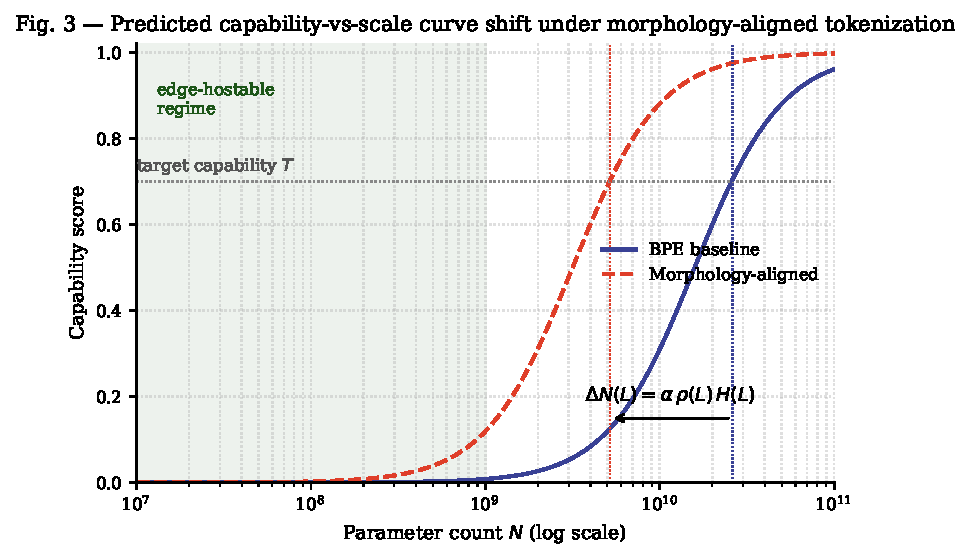
\includegraphics[width=0.78\linewidth]{fig_03_curve_shift_schematic.pdf}
\vspace{-0.3\baselineskip}
\caption{Predicted capability-vs-scale curve shift under morphology-aligned tokenisation (Equation~\ref{eq:curveshift}). The framework is neutral between sharp-emergence \citep{wei2022} and smooth-improvement \citep{schaeffer2023} readings of the capability-vs-scale curve; only the magnitude of the shift $\Delta N(L)$ is predicted.}
\label{fig:curve-shift}
\end{figure}
\FloatBarrier

\section{Case Studies}
\label{sec:cases}

\S\ref{sec:framework} developed the framework abstractly. \S\ref{sec:results} reports what the four-language experiment observed. This section connects the two. For each of the four languages tested, we describe the morphological system at the level of organisation relevant to the framework, walk through how the grammar engine decomposes representative word forms, and report the numerical inputs ($|B(L)|$, $H(L)$, $\rho(L)$) that the engine produces from a 20{,}000-sentence sample of the mixed Wikipedia and FineWeb corpora. The four subsections follow the project's canonical order (Mandarin, English, Turkish, Arabic), from the most isolating system to the most templatic, the order in which the framework predicted the rebate would grow, a prediction \S\ref{sec:results} puts to the test and, for three of the four languages, overturns.

\subsection{Mandarin: isolating}
\label{sec:cases-zh}

Mandarin sits at the isolating end of the typological spectrum. Grammar is carried by word order and a small inventory of function words, and inflectional morphology in the European sense is essentially absent: verbs do not conjugate for person or tense, nouns do not decline for case, and most words consist of a single morpheme or a stable two-character compound. Grammatical relations that European languages bundle into suffixes are instead handled by free particles: aspect is marked by post-verbal \emph{le} (\zh{了}, perfective), \emph{zhe} (\zh{着}, durative), and \emph{guo} (\zh{过}, experiential); argument structure is rearranged by the \emph{ba} construction (\zh{把}); modality is carried by pre-verbal auxiliaries such as \emph{hui} (\zh{会}, ``will / be able to'') and \emph{neng} (\zh{能}, ``can'').

But Mandarin carries its own structural signal, hidden at a layer below the word. Every Han character is built around a \emph{Kangxi radical}, the semantic component used to organise the traditional dictionary. The radical encodes a coarse semantic class: \zh{子} marks CHILD / KINSHIP terms, \zh{木} marks TREE / WOOD entities, \zh{水} (and its combining form \zh{氵}) marks WATER / LIQUID, \zh{心} (and \zh{忄}) marks HEART / EMOTION, \zh{言} (and \zh{讠}) marks SPEECH / LANGUAGE, and so on across the 214-radical Kangxi system. This radical-semantic axis is the structural analog of Arabic's \emph{wazn}-semantic-class axis: in both languages, a non-concatenative layer of semantic information sits behind the surface form, and a tokeniser that knows to look at it gains access to a signal that flat byte-level segmentation discards.

A representative decomposition: the word \zh{学习} (\emph{xu\'exi}, ``to study'') decomposes into two characters, each carrying its own radical. \zh{学} (\emph{xu\'e}, ``learn'') is built on radical \zh{子} (CHILD), placing it in the HUMAN\_RELATION semantic class; \zh{习} (\emph{x\'i}, ``practise'') is built on radical \zh{羽} (FEATHERS), placing it in the NATURAL\_OBJECT class. The compound is grammatically a verb, but its grammatical identity sits in syntactic position rather than in any inflectional marker on the form itself; aspectual nuance, when needed, is supplied by a following particle (\zh{了}, \zh{着}, \zh{过}).

Mandarin's structural bundle ceiling is $|B(L)| = 547$ ($H_{\max} \approx 9.10$ bits); the full corpus attests $131$ distinct bundles, populated by part-of-speech, particle-class, and radical-class combinations rather than by inflection. Two of the engine's numbers for Mandarin must be read with care. The raw $H(L) = 6.28$ bits is anomalously high for an isolating language that marks almost no grammar on the word; it reflects the breadth of the character-and-radical serialisation, not a genuine inflectional load, and tightening the Mandarin bundle definition so that $H$ measures grammar rather than serialisation breadth is noted as engine work in \S\ref{sec:conclusion}. What is linguistically meaningful is the structural recoverability, $\rho(\text{Mandarin}) \approx 0.025$: almost none of what the engine serialises is recoverable from the bare character string, because Mandarin's grammar lives in word order and free particles, not on the word surface. The product $\rho(L)\cdot H(L) \approx 0.16$, the lowest of the four, is therefore correct despite the inflated $H$: Mandarin exposes the least surface grammar. The \texttt{radical\_class} stream adds a separate, lexicon-recoverable semantic axis: 214 Kangxi radicals in principle, some 30 covering most of the corpus.

\subsection{English: analytic}
\label{sec:cases-en}

English is the next-most analytic of the four languages, and the typological baseline against which the framework's predictions will feel least surprising. English grammar is carried largely by word order and by function words (articles, prepositions, auxiliaries). Inflectional morphology is limited to a small inventory of suffixes (plural \emph{-s}, possessive \emph{'s}, third-person-singular present \emph{-s}, past \emph{-ed}, progressive \emph{-ing}, comparative \emph{-er}, superlative \emph{-est}), plus a closed set of suppletive and irregular forms (\emph{go/went}, \emph{be/was}, \emph{child/children}) resolved through a lookup list. Derivational morphology is richer, and the engine now treats it as a productive layer rather than a lexicalised annotation: affixes are peeled off the surface form, one at a time, until a known root is reached.

A representative decomposition. The word \emph{researchers} resolves to root \emph{search}, a derivational chain \texttt{[er $\to$ AGENT\_NOUN, re $\to$ REPETITION]}, and feature bundle \texttt{pos=NOUN | num=PL}. Each derivational affix is annotated by the semantic role it contributes, rather than collapsed into a lexicalised stem. The word \emph{went} resolves to the suppletive root \emph{go} with bundle \texttt{pos=VERB | tense=PAST}; the surface string bears no phonological relationship to its root, and the lookup list is the only route by which the underlying form is recovered. The word \emph{runs} is ambiguous on the surface alone between a plural noun and a third-person-singular verb; the engine resolves this through part-of-speech inference and records the residual ambiguity with an \texttt{ambig\_3sg=YES} tag.

The feature-bundle inventory remains small. English's structural ceiling is $|B(L)| = 89$, with $H_{\max}(L) = \log_2 89 \approx 6.48$ bits; the full corpus attests only $21$ distinct bundles. The corpus-weighted grammatical entropy is $H(L) = 1.30$ bits per word. The wide gap between $H(L)$ and $H_{\max}(L)$ reflects the strong peakedness of English's bundle distribution: most English word forms are uninflected singular nouns or bare verbs, and the entropy of their features is correspondingly low.

Surface ambiguity in English is localised and well-bounded. The \emph{-s} homograph between noun plural and verb 3SG, identified through corpus statistics, is the main contributor to $H(b \mid \text{signature})$. The signature-conditional entropy comes to $0.23$ bits; $\rho(\text{English}) = 1 - 0.23 / 1.30 \approx 0.82$. English therefore exposes roughly four-fifths of its grammatical information on the surface form, a high recoverability limited chiefly by irregular forms and by the handful of genuinely ambiguous surface patterns.

The framework's predicted ordering variable for English is $\rho \cdot H \approx 1.07$ bits, second-smallest of the four, predicting a small rebate. \S\ref{sec:results} reports something stronger than a small rebate, namely none: at compute-optimal scale English's grammar-aware model finishes $\Delta\mathrm{bpc} = -0.036$, \emph{worse} than its baseline. English's grammar is legible enough from the surface that a model with sufficient data learns it unaided, and the explicit feature stream only adds cost.

\subsection{Turkish: agglutinative}
\label{sec:cases-tr}

Turkish is the framework's cleanest case. Its word forms are built by stacking suffixes onto a root in a strict slot order: root $\to$ derivational markers $\to$ number $\to$ possessive $\to$ case for nouns, and root $\to$ derivational markers $\to$ voice $\to$ tense/aspect/mood $\to$ person for verbs. Vowel harmony adjusts the surface shape of each suffix to match the vocalic profile of the root, but the harmony rules are regular and invertible; feature tags are harmony-normalised, so \emph{-den} and \emph{-dan} both carry the single tag \texttt{case=ABL}. Morpheme boundaries are unambiguous, and the slot-order constraint rules out combinatorial ambiguity. The engine now performs a holistic verbal and nominal analysis, with deterministic tie-breaks, so that competing analyses of an ambiguous suffix string resolve to a single canonical parse. Two refinements matter for the corpus statistics. A proper-noun fallback intercepts capitalised sentence-initial tokens (\emph{Ahmet}, \emph{\.{I}stanbul}, \emph{T\"urkiye}) and labels them \texttt{pos=PROPN} with an empty bundle, rather than forcing them through the verbal analyser and producing spurious tense and person tags. And denominal-verb derivations in \emph{-le} and \emph{-la\c{s}} (\emph{ba\c{s}-la}, ``to begin''; \emph{g\"uzel-le\c{s}}, ``to become beautiful'') are recognised as a derivational layer before inflectional peeling, so that the verbal bundle attaches to a derived verbal stem rather than to the underlying nominal root.

A representative decomposition. The word \emph{evlerinizden} (``from your (pl.) houses'') resolves to root \emph{ev} (``house'') and feature bundle \texttt{pos=NOUN | num=PL | poss=2PL | case=ABL}, a four-slot stack (plural marker \emph{-ler}, second-person-plural possessive \emph{-iniz}, ablative case \emph{-den}). The word \emph{yaz{\i}ld{\i}} (``it was written'') resolves to root \emph{yaz} (``write'') and bundle \texttt{pos=VERB | voice=PASS | tense=PAST\_DEF}. The surface string is the concatenation of the root and the ordered suffix sequence; for well-formed text, the engine's parse is the unique analysis consistent with the slot-order grammar.

The feature-bundle inventory is large, reflecting the combinatorial nature of Turkish agglutination. Turkish's structural ceiling is $|B(L)| = 4{,}382$, with $H_{\max} = \log_2 4382 \approx 12.10$ bits; the full corpus attests $469$ distinct bundles, and the corpus-weighted entropy is $H(L) = 4.01$ bits. Each slot admits several values, and their Cartesian product yields a large effective space even at moderate per-slot cardinality; a proper-noun fallback keeps the count from inflating further by collapsing the long tail of \emph{Ahmet}, \emph{\.{I}stanbul}, \emph{T\"urkiye}-type capitalised forms into a single \texttt{PROPN} signature rather than forcing each through the verbal analyser. The gap between $H_{\max}$ and $H(L)$ reflects the corpus distribution's concentration on a smaller subset of frequently-used combinations.

Structural recoverability is Turkish's distinguishing property. The conditional entropy $H(b \mid \text{signature})$ on the 20{,}000-sentence sample is $1.03$ bits, yielding $\rho(\text{Turkish}) = 1 - 1.03/4.01 \approx 0.74$. Turkish does not reach $\rho = 1$: vowel-harmony variant classes, a small number of irregular verbal stems, and some derivational homographies leave residual surface ambiguity. But $\rho$ for Turkish sits high, close to English's $0.82$ and well above Arabic's $0.53$, confirming that Turkish wears its grammar on the surface.

The framework's predicted ordering variable for Turkish is $\rho \cdot H \approx 2.98$ bits, second only to Arabic. Turkish was, on the strength of its typology, the language we most expected to gain. A cleanly agglutinative system stacks its grammar in transparent, surface-recoverable suffixes, exactly the configuration the framework rewards, and the small-scale pilot's early impression pointed the same way, with Turkish the most promising of the three pilot languages (\S\ref{sec:results-pilot}). On typological grounds Turkish was the natural poster case, the language whose structure should make grammar-aware tokenisation pay most.

That expectation does not survive scale. At the compute-optimal, parameter-matched scale of \S\ref{sec:results}, Turkish's rebate is gone: $\Delta\mathrm{bpc} = -0.017$, the grammar-aware model finishing \emph{worse} than its baseline despite carrying more parameters and a larger vocabulary. The very transparency that made Turkish the framework's poster case turns out to be its undoing here: because Turkish wears its grammar openly on the surface, a model given enough data simply learns that morphology for itself, and handing it the same suffix analysis explicitly buys nothing while costing a little. Turkish's fall, from the pilot's early promise to no rebate at compute-optimal scale, is the clearest single sign that the Agglutinative Compounding Effect was an artefact of under-training rather than a property of agglutinative structure. The prediction the framework got right was a ranking the pilot's impression anticipated; the prediction it got wrong was that the ranking would mean anything once the baselines were properly trained.

\subsection{Arabic: templatic}
\label{sec:cases-ar}

Arabic's morphological system is organised around two orthogonal axes: a consonantal root carrying semantic content (predominantly three consonants, with a smaller class of quadriliteral roots and a handful of longer ones), and a pattern (\ar{وَزْن}, \emph{wazn}) carrying grammatical content. The root combines, in strict consonantal order, with any of a fixed set of patterns to produce a family of related words, each interleaving the root consonants with pattern-specific vowels and affixes. The root \ar{ك-ت-ب} (\emph{k-t-b}, the writing-related meaning) combines with pattern~I to give \ar{كَتَبَ} (\emph{kataba}, ``he wrote''); with pattern~III to give \ar{كَاتَبَ} (\emph{k\=ataba}, ``he corresponded with''); and with the active-participle pattern of form~I to give \ar{كَاتِب} (\emph{k\=atib}, ``writer''). The same consonantal skeleton runs through all of these; the grammatical identity sits in the pattern.

The engine represents Arabic word forms through a four-part decomposition: the surface string, a feature bundle, the extracted triconsonantal root, and a \emph{wazn-class} label that names the semantic role of the pattern. The wazn-class taxonomy partitions the templatic system into 185 semantic classes, capturing the regularity that each Arabic pattern is associated with a recognisable semantic effect on its root (causative, intensive, reciprocal, seeking, and so on). A representative decomposition. The word \ar{اسْتَخْدَمَ} (\emph{istakhdama}, ``he used'') resolves to root \ar{خ-د-م} (\emph{kh-d-m}, the serving-related meaning), feature bundle \texttt{pos=VERB | form=X}, and wazn-class \texttt{FORM\_X\_SEEKING} (the SEEKING\_ESTIMATIVE / REQUEST role, in which Form~X derives a verb of seeking, requesting, or considering-to-be from its base; \emph{istakhdama} therefore reads literally as ``he sought service from'' before lexicalising to ``he used''). The word \ar{الْمِصْرِيَّة} (\emph{al-mi\d{s}riyya}, ``the Egyptian (feminine)'') resolves to root \ar{مِصْر} (\emph{m-\d{s}-r}, Egypt), bundle \texttt{pos=NOM | def=DEF | role=DERIVED}, and the corresponding nominal wazn-class. Arabic prefixes and suffixes (the definite article \ar{الْـ}/\emph{al-}, person markers on verbs, gender and number agreement markers on nouns) appear alongside the pattern as tag values rather than as independent morphemes. The engine propagates the \texttt{semantic\_role} field into the bundle through a lookup step (Step~B$'$, the wazn-class resolver) that runs after templatic identification. It is this propagation layer that turns the templatic-lexical-surplus prediction from a theoretical claim into a testable one.

The feature-bundle inventory is the largest of the four. Arabic's structural ceiling is $|B(L)| = 9{,}579$, with $H_{\max} = \log_2 9579 \approx 13.23$ bits; the full corpus attests $1{,}450$ distinct bundles, and the corpus-weighted entropy is $H(L) = 6.51$ bits. The high $H(L)$ reflects Arabic's rich grammatical encoding: gender, number, definiteness, case, person, aspect, voice, templatic form, and wazn-class semantic role all live on a single word form, and their realised distribution in natural text is less concentrated than the other languages'.

Structural recoverability is where Arabic's typological character asserts itself most clearly. The observed conditional entropy $H(b \mid \text{signature})$ is $3.04$ bits, far higher than English's $0.23$ or Turkish's $1.03$. This follows from the inherent ambiguity of the templatic system: the engine's template labels collapse many distinct feature bundles into the same surface pattern. For instance, \texttt{VERB\_TRILATERAL\_BARE} is carried by forms of many tense, voice, and agreement combinations, which the template alone cannot distinguish without lexical or contextual resolution. $\rho(\text{Arabic}) = 1 - 3.04/6.51 \approx 0.53$. Only about half of Arabic's grammatical information is recoverable from the surface-pattern signature; the other half requires lexicon access or context. Arabic has, by a wide margin, the lowest $\rho$ of the four languages, the formal statement of the fact that it hides more of its grammar off the surface than any of the others.

The framework's predicted ordering variable for Arabic is $\rho \cdot H \approx 3.47$ bits, the highest of the four. Arabic is the one language for which grammar-aware tokenisation pays at compute-optimal scale: \S\ref{sec:results} records $\Delta\mathrm{bpc} = +0.0192 \pm 0.0023$ (the mean over four seeds), the only positive rebate of the four. The reason is the low $\rho$ rather than the high $\rho \cdot H$. The half of Arabic's grammar that sits off the surface is precisely what a surface-reading model cannot learn from text on its own, so the explicit root and \emph{wazn} streams supply information that is otherwise out of reach. This is the Templatic Lexical Surplus; whether it is the templatic structure or merely the parameters those streams add that earns the rebate is settled by the ablation of \S\ref{sec:results-ablation}.


\section{Empirical Results}
\label{sec:results}

\S\ref{sec:framework} issued two predictions. In its rank form, the framework holds that the parameter rebate from grammar-aware tokenisation over a byte-pair baseline is ordered across languages by $\rho(L) \cdot H(L)$. In its magnitude form, it holds that a single coefficient $\alpha$ turns that product into a quantitative prediction. The main test is a four-language experiment, Mandarin, English, Turkish, and Arabic, parameter-matched in the transformer and trained at the compute-optimal budget. We report it first (\S\ref{sec:results-design}--\S\ref{sec:results-phase2}), then summarise in brief the smaller three-language pilot (\S\ref{sec:results-pilot}) that motivated it.

\subsection{Design}
\label{sec:results-design}

For each of the four languages we train one baseline and one grammar-aware model, identical in architecture, optimiser, data, and training budget, differing only in the tokeniser. Each is a decoder-only transformer with 512-dimensional embeddings, 10 layers, 8 attention heads, and a 128-token context, holding approximately $3.2 \times 10^7$ parameters in the transformer the two regimes share. Each trains for $6.4 \times 10^8$ tokens, close to the compute-optimal twenty tokens per parameter \citep{hoffmann2022}, placing the comparison inside the regime where the Hoffmann coefficients were fitted. The grammar-aware variant adds the feature-bundle stream summed at the input layer (\S\ref{sec:framework-engine}), with two further streams, the consonantal root and the \emph{wazn} pattern, for Arabic. One asymmetry must be stated plainly, because it bears on the reading of the result: the baseline tokeniser uses a 32k vocabulary while the grammar-aware surface stream uses 50k, and each additional stream carries its own embedding table. The grammar-aware models therefore hold \emph{more} parameters than their baselines, from $45.0$M (Mandarin) up to $70.7$M (Arabic) against the baselines' $44.9$--$48.0$M (Table~\ref{tab:phase2}). This is the same vocabulary-and-parameter asymmetry the pilot flagged, and it favours the grammar-aware regime; a negative result for that regime is therefore conservative, and the one positive result, Arabic, is exactly the case where we must rule the asymmetry out (\S\ref{sec:results-phase2}, and the ablation in \S\ref{sec:conclusion}).

\paragraph{Corpora.} To give every language the broadest variety of text, and to lift Turkish above the ceiling a Wikipedia-only corpus imposes, each language draws from two registers: encyclopaedic Wikipedia and large-scale web crawl (FineWeb for English, FineWeb-2 for the others). Five million sentences per language were sampled, deduplicated, and interleaved. Table~\ref{tab:phase2-corpus} reports the resulting training-token counts. One consequence of holding the token budget fixed across corpora of different size must be flagged: at $6.4 \times 10^8$ tokens the models see their unique training text roughly once for Mandarin, but about four times for Arabic, five for English, and seven for Turkish. Epoch count is therefore not matched across languages. It is a confound we cannot remove post hoc, and it bears on any cross-language reading of the deltas, since heavier repetition tends to raise held-out loss; it is revisited in \S\ref{sec:discussion-limitations}.

\begin{table}[hbt!]
\centering
\small
\begin{tabular}{lrr}
\toprule
Language & Train tokens & Source characters \\
\midrule
Mandarin & $6.34 \times 10^8$ & $6.44 \times 10^8$ \\
English  & $1.18 \times 10^8$ & $6.58 \times 10^8$ \\
Turkish  & $8.88 \times 10^7$ & $5.97 \times 10^8$ \\
Arabic   & $1.51 \times 10^8$ & $8.33 \times 10^8$ \\
\bottomrule
\end{tabular}
\caption{Phase~2 training corpora, mixed Wikipedia and FineWeb, five million sentences per language. The Turkish count is roughly thirty times the pilot corpus, removing the data-starvation confound at the agglutinative pole.}
\label{tab:phase2-corpus}
\end{table}
\FloatBarrier

\paragraph{Metric: bits per character.} Per-token cross-entropy is not comparable across tokenisers whose segmentations differ, because a model that emits fewer, longer tokens is scored on fewer but harder predictions. We therefore report the tokeniser-neutral quantity
\[
\mathrm{bpc} = \frac{\mathcal{L}}{\ln 2} \cdot \frac{T}{C},
\]
the cross-entropy $\mathcal{L}$ in nats per token, converted to bits and rescaled by the ratio of tokens $T$ to source characters $C$ on the held-out set. Bits per character scores the cost of the text itself and is directly comparable between baseline and grammar-aware regimes.

\subsection{The four-language result}
\label{sec:results-phase2}

Table~\ref{tab:phase2} reports the headline result. Of the four languages, three show no rebate and one does; Figure~\ref{fig:p2-rebate} shows the same result graphically.

\begin{table}[hbt!]
\centering
\small
\begin{tabular}{lrrrrr}
\toprule
Language & $\rho \cdot H$ & $\mathrm{bpc}_\mathrm{BPE}$ & $\mathrm{bpc}_\mathrm{morph}$ & $\Delta\mathrm{bpc}$ & params (base\,$\to$\,morph) \\
\midrule
Mandarin & 0.16 & 4.3795 & 4.3839 & $-0.0044$ & 44.9\,M\,$\to$\,45.0\,M \\
English  & 1.07 & 1.0527 & 1.0883 & $-0.0356$ & 48.0\,M\,$\to$\,57.2\,M \\
Turkish  & 2.98 & 0.8811 & 0.8976 & $-0.0165$ & 48.0\,M\,$\to$\,58.2\,M \\
Arabic   & 3.47 & 1.1464 & 1.1246 & \textbf{$+0.0218$} & 48.0\,M\,$\to$\,70.7\,M \\
\bottomrule
\end{tabular}
\caption{Four-language result in bits per source character, at $\approx 32$M matched transformer parameters and compute-optimal training. Positive $\Delta\mathrm{bpc}$ favours the grammar-aware regime. Only Arabic shows a rebate; the three deltas of the surface-legible languages are negative and are not ordered by $\rho \cdot H$.}
\label{tab:phase2}
\end{table}
\FloatBarrier

\begin{figure}[hbt!]
\centering
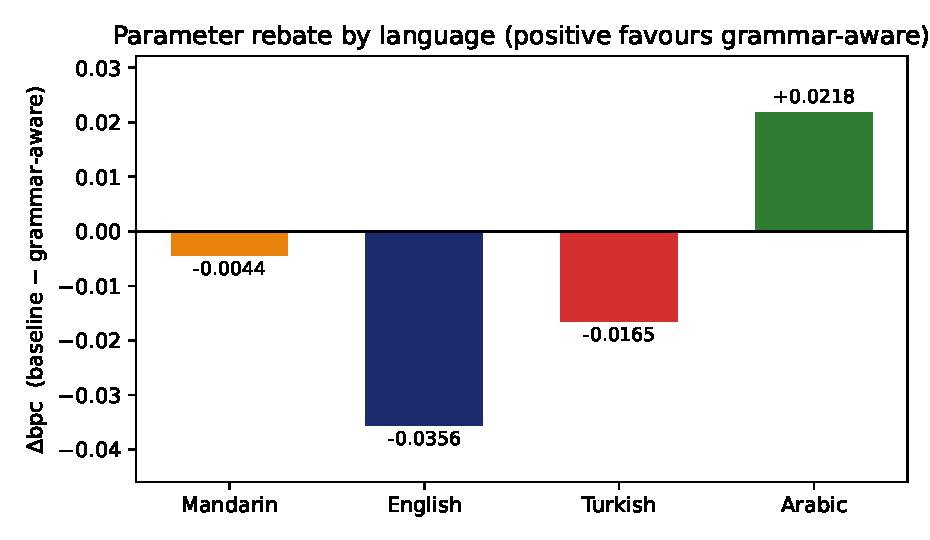
\includegraphics[width=0.82\linewidth]{fig_p2_rebate.pdf}
\caption{Parameter rebate $\Delta\mathrm{bpc}$ (baseline $-$ grammar-aware) by language, at compute-optimal, transformer-matched scale. Only Arabic, the templatic case, shows a positive rebate; the three surface-recoverable languages fall below zero. Colours follow the project convention: Mandarin orange, English navy, Turkish red, Arabic green.}
\label{fig:p2-rebate}
\end{figure}
\FloatBarrier

\paragraph{The ordinal prediction fails.} The framework predicts that $\Delta\mathrm{bpc}$ rises with $\rho \cdot H$. It does not. Mandarin, English, and Turkish all land on the wrong side of zero ($-0.004$, $-0.036$, $-0.017$), and their order bears no relation to $\rho \cdot H$: English, in the middle of the range, is the most negative, and Turkish, the agglutinative case in which the framework predicts the largest rebate, shows none. At compute-optimal, parameter-matched scale, the rank prediction that survived the pilot does not survive here. This is the outcome the pilot's Interpretation~B anticipated for the surface-recoverable languages: a model trained on enough data learns their grammar from the text itself, so handing it the same grammar as an explicit input is redundant, and the extra input streams, far from helping, cost a little. Figure~\ref{fig:p2-prediction} makes the failure visual: plotted against the engine's $\rho \cdot H$, the four rebates show no monotonic trend.

\begin{figure}[hbt!]
\centering
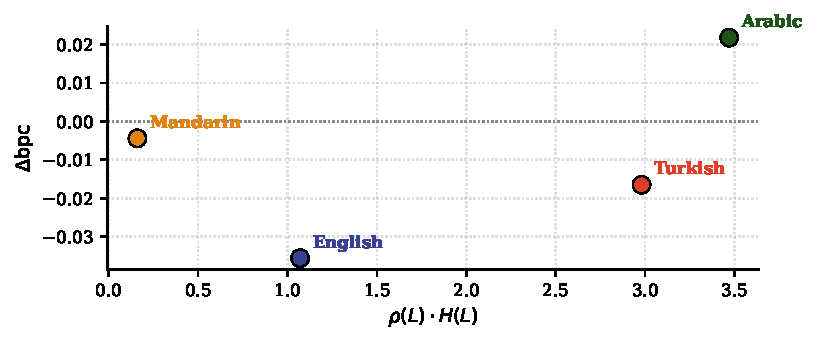
\includegraphics[width=0.75\linewidth]{fig_p2_prediction.pdf}
\caption{Observed rebate against the framework's pre-registered predictor $\rho(L)\cdot H(L)$. The framework predicts the rebate should rise with $\rho \cdot H$; instead three languages sit below zero in no particular order and only Arabic is positive. The surviving signal tracks low $\rho$ (off-surface grammar), not high $\rho \cdot H$.}
\label{fig:p2-prediction}
\end{figure}
\FloatBarrier

\paragraph{Arabic is the exception, and it is the informative one.} Arabic alone delivers a rebate: $+0.0218$ bpc in the primary run of Table~\ref{tab:phase2}, replicated at $+0.0192 \pm 0.0023$ bpc across four seeds (\S\ref{sec:results-seeds}). What sets Arabic apart is not that its $\rho \cdot H$ is highest, but that its $\rho$ is \emph{lowest} ($0.534$): more of its grammar is hidden off the written surface, locked in the interleaving of consonantal root and vocalic pattern, than in any of the other three. That is precisely the grammatical information a surface-reading model cannot reconstruct on its own, no matter how much text it sees, because it is not on the surface to be read. When the root and \emph{wazn} streams hand that hidden structure to the model directly, it helps. The rebate, in other words, appears to track the \emph{unrecoverable} fraction of grammar rather than the recoverable product $\rho \cdot H$ the framework was built on, a reading we develop and heavily qualify in \S\ref{sec:discussion-reformulated} (it is a conjecture from one positive language, not a fitted law).

This is the \textbf{Templatic Lexical Surplus} (\S\ref{sec:results-pilot}), reproduced here at compute-optimal scale, standing where the broader rebate has dissolved. The learning curves (Figure~\ref{fig:p2-curves}) show the divergence directly: the grammar-aware trace runs above its baseline throughout for Mandarin, English, and Turkish, and below it for Arabic alone.

\begin{figure}[hbt!]
\centering
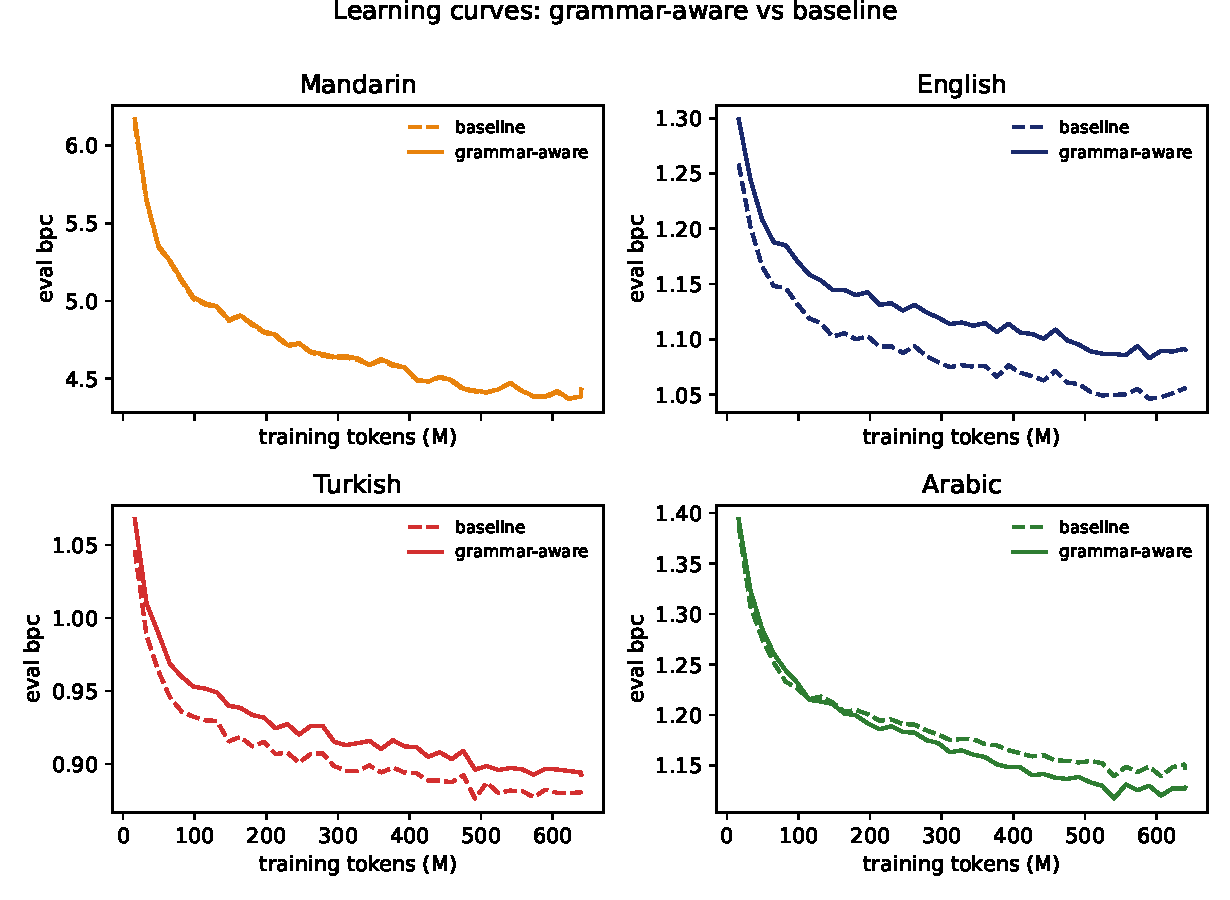
\includegraphics[width=0.78\linewidth]{fig_p2_curves.pdf}
\caption{Evaluation bits per character against training tokens, grammar-aware (solid) versus baseline (dashed), per language. Lower is better, so the grammar-aware model helps only when its solid trace sits \emph{below} the dashed one, which happens for Arabic alone.}
\label{fig:p2-curves}
\end{figure}
\FloatBarrier

\paragraph{A capacity caveat.} The Arabic comparison is parameter-matched in the transformer but not in total: the root and \emph{wazn} embedding tables raise the Arabic grammar-aware model to $70.7$M parameters against the baseline's $48.0$M, a rise of roughly one half. Part of Arabic's rebate could in principle be bought by that extra capacity rather than by the structure the streams encode. Two observations bound the worry but do not dispel it. English and Turkish carry extra parameters too ($+19\%$ and $+21\%$) and gain nothing, which argues against a pure-capacity reading; and the framework's own estimate of the embedding cost (\S\ref{sec:framework-A1}) treated it as negligible, an assumption these counts show to be too generous for the four-stream Arabic case. A parameter-matched ablation is the one experiment that would convert this result from suggestive to clean; we run it, and we explain why we run it for Arabic alone, in \S\ref{sec:results-ablation}.

\subsection{Isolating structure from capacity: the Arabic ablation}
\label{sec:results-ablation}

The single positive result, Arabic, is also the one most exposed to a capacity objection, since its grammar-aware model carries roughly half as many parameters again as its baseline. We therefore control for capacity directly, and we do so for Arabic alone. The choice is dictated by the result, not by the language, and the reasoning should be made explicit because the one language that gained happens to be the first author's native tongue. A capacity confound can only manufacture a \emph{positive} effect; it cannot conceal one. The three languages that show no rebate carry the same kind of parameter surplus, and a larger surface vocabulary besides, so the extra capacity is working \emph{in their favour} and they lose regardless; their null results are therefore conservative, and controlling for capacity could only deepen them. Arabic is the only language whose extra parameters might be doing the work we would otherwise credit to structure, so it is the only language where the control carries information. The identical criterion would have singled out whichever language came out positive; that it is Arabic changes neither the rule nor its application.

The control holds the Arabic grammar-aware model fixed in every respect, architecture, parameter count, token budget, and optimiser, and randomises only the \emph{content} of the root and \emph{wazn} streams: each position receives a root and a pattern drawn from the corpus distribution but decoupled from the word actually present. The streams thus cost exactly the same parameters while carrying no real templatic information. If Arabic's rebate is structural, the model with true root and \emph{wazn} streams should beat this shuffled control; if the rebate is merely capacity, the two should tie. The outcome is decisive, and in the structural direction. The shuffled control finishes at $1.1676$ bpc, not merely worse than the real grammar-aware model ($1.1246$) but worse than the baseline itself ($1.1464$). Randomising the root and \emph{wazn} streams, while holding their parameters exactly, does not just erase Arabic's rebate: it turns the two streams into noise that costs $0.021$ bpc against baseline. The real templatic streams therefore outperform identically-sized random ones by $0.043$ bpc. Capacity is not merely an insufficient explanation for Arabic's rebate; added capacity \emph{without} real structure is actively harmful, and the whole of the rebate, indeed more than it, is attributable to the templatic information the streams carry. The Templatic Lexical Surplus, on this test, is a structural effect and not a parameter artefact. Figure~\ref{fig:p2-ablation} shows the three Arabic models side by side.

\begin{figure}[hbt!]
\centering
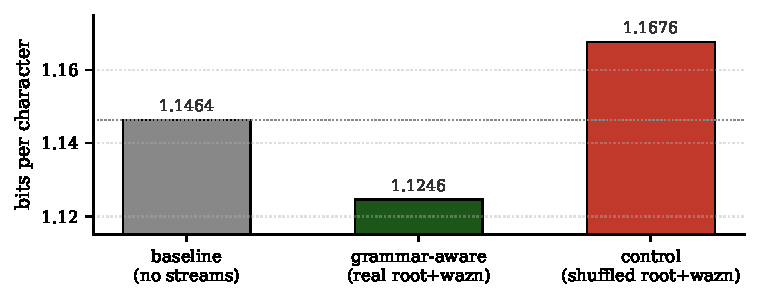
\includegraphics[width=0.82\linewidth]{fig_p2_ablation.pdf}
\caption{The Arabic ablation, in bits per character (lower is better). The grammar-aware model with real root and \emph{wazn} streams beats the baseline; the same model with those streams \emph{shuffled}, at identical parameter count, falls \emph{below} the baseline. The rebate is the templatic information, not the parameters carrying it.}
\label{fig:p2-ablation}
\end{figure}
\FloatBarrier

\subsection{Robustness across random seeds}
\label{sec:results-seeds}

A single training run cannot separate a real effect of this size from the luck of one random initialisation and one data ordering. We therefore re-ran the Arabic comparison, baseline, grammar-aware, and shuffled control, across four independent random seeds. The rebate is stable: the grammar-aware model beats the baseline in all four seeds, by $0.0192 \pm 0.0023$ bits per character (mean $\pm$ standard deviation), a margin roughly eight times its own run-to-run scatter. The structural control is stable too: the real root and \emph{wazn} streams beat their shuffled counterparts by $0.0429 \pm 0.0007$ bpc, and the shuffled model finishes below the baseline in every seed. Figure~\ref{fig:p2-seeds} shows the three regimes with their seed-level spread. The effect is small in absolute terms but robust: it survives replication, and the shuffle control locates it in the templatic structure rather than in the parameters the streams add.

\begin{figure}[hbt!]
\centering
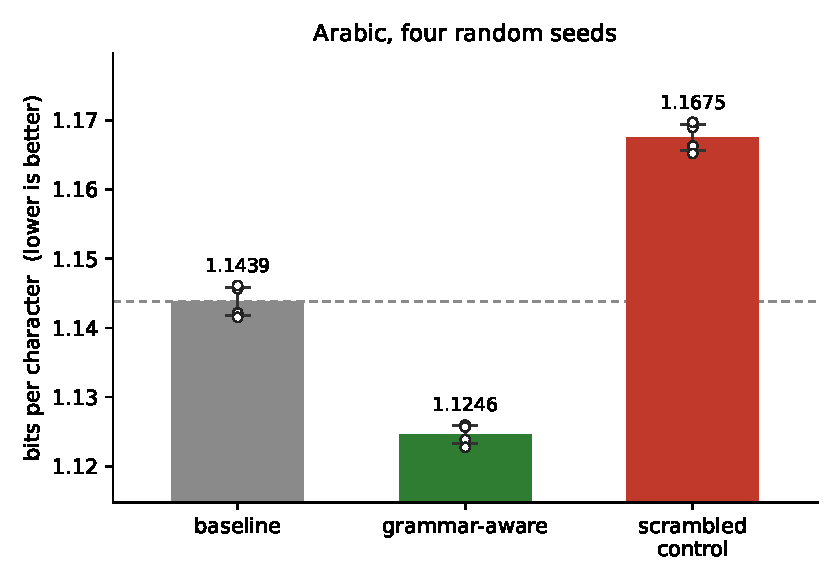
\includegraphics[width=0.82\linewidth]{fig_p2_seeds.pdf}
\caption{Arabic across four random seeds, in bits per character (lower is better). Bars are seed means, whiskers the spread. The grammar-aware model (real root and \emph{wazn}) is lowest; the scrambled-control model, at identical parameter count, is highest, worse even than the byte-pair baseline. Both the grammar-aware rebate ($+0.0192 \pm 0.0023$ bpc) and its margin over the scrambled control ($+0.0429 \pm 0.0007$ bpc) hold across all four seeds.}
\label{fig:p2-seeds}
\end{figure}
\FloatBarrier

\subsection{The three-language pilot, in brief}
\label{sec:results-pilot}

The study grew out of a budget-limited pilot run in mid-May 2026: six decoder-only models, one baseline and one morphology-aligned pair for each of English, Arabic, and Turkish, at roughly $2 \times 10^6$ parameters and $5 \times 10^6$ training tokens, about eight times below the compute-optimal budget, and scored with the pre-reform engine's coarser bundle counts. The pilot was an impression-gathering exercise, not a controlled measurement: at that scale, the test-loss reduction under morphology-aligned tokenisation appeared to track the engine's $\rho \cdot H$ ordinal prediction, an impression that motivated the four-language study reported above rather than a result to be quoted on its own terms. It also suggested a magnitude puzzle, an apparent growth of the per-bit rebate with $\rho \cdot H$ that we provisionally named the \textbf{Agglutinative Compounding Effect}; at this scale, and with an engine later substantially revised for real-text accuracy, the pattern is best read as a prompt for further work rather than a measured quantity. Figure~\ref{fig:pilot-ordinal} shows the pilot's early impression.

\begin{figure}[hbt!]
\centering
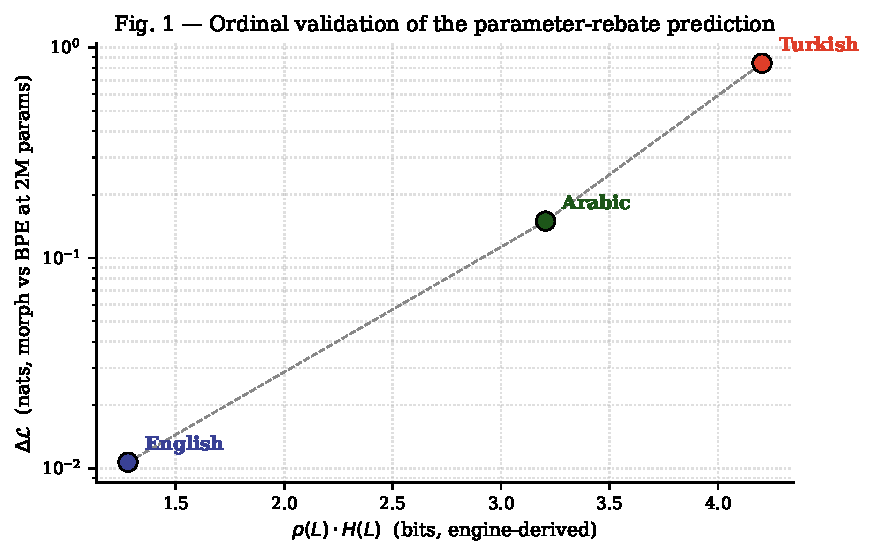
\includegraphics[width=0.72\linewidth]{fig_01_ordinal_validation.pdf}
\caption{The pilot's early impression (three languages, $\sim$2M parameters, mid-May 2026, pre-reform engine). At this exploratory scale, the reduction in test loss under morphology-aligned tokenisation appeared to track the engine's $\rho \cdot H$ ordinal prediction, motivating the four-language experiment reported above. \S\ref{sec:results-phase2} shows that this impression does not survive at compute-optimal, parameter-matched scale with the reformed engine.}
\label{fig:pilot-ordinal}
\end{figure}
\FloatBarrier

A three-rung scale ladder toward compute-optimal training already hinted that the effect was scale-fragile: the English and Arabic rebates inverted as the rungs grew, while Turkish's held at this exploratory scale. The pilot could not decide whether these inversions meant the rebate was a genuine artefact of under-training (Interpretation~B) or whether a confound was masking a real effect, because the morphology-aligned models also carried a larger vocabulary, and so more parameters, than their baselines. A separate, exploratory Arabic probe that added an explicit consonantal-root stream on top of surface morphology hinted at a small additional rebate persisting across the ladder, the germ of the observation we later name the \textbf{Templatic Lexical Surplus}. The four-language experiment was designed to settle the pilot's open questions properly: at compute-optimal scale, with the reformed engine, and with the vocabulary-cap asymmetry removed. It does: the impression of an Agglutinative Compounding Effect does not survive, while the Templatic Lexical Surplus does, now measured cleanly rather than glimpsed.

\subsection{Summary}
\label{sec:results-summary}

At compute-optimal, transformer-matched scale, grammar-aware tokenisation delivers no parameter rebate for Mandarin, English, or Turkish, and the framework's $\rho \cdot H$ ordering does not hold. The pilot's Agglutinative Compounding Effect is, for these surface-recoverable languages, an artefact of under-training: once a model has enough data to learn grammar from the text, being handed that grammar explicitly is redundant. Arabic is the single exception. Its templatic morphology stores grammar off the surface, where a surface-reading model cannot recover it at any scale, and exposing that structure through explicit root and \emph{wazn} streams lowers its bits per character by $0.0192 \pm 0.0023$ (the mean over four seeds). The surviving signal therefore tracks the \emph{unrecoverable} grammar a language hides, not the recoverable grammar the original framework measured, and it reproduces the pilot's Templatic Lexical Surplus at proper scale. The one capacity confound, the extra parameters the Arabic streams cost, is resolved directly by the shuffle-control ablation of \S\ref{sec:results-ablation}: identically-sized streams filled with random root and \emph{wazn} content perform worse than the baseline, so Arabic's rebate is the templatic structure itself, not the parameters that carry it.

\section{Discussion}
\label{sec:discussion}

\S\ref{sec:results-summary} summarised the split verdict; this section asks what it means. We take the two halves in turn, Turkish's collapsed rebate and Arabic's surviving one, then draw out the consequences and the limits.

\subsection{The Agglutinative Compounding Effect does not survive scale}
\label{sec:discussion-ace}

The pilot's headline phenomenon, the apparent super-linear growth of the rebate with $\rho \cdot H$, is not reproduced (\S\ref{sec:results-phase2}). Turkish is the decisive case: the cleanest agglutinative system in the set, the language both the typology and the pilot's early impression favoured most (\S\ref{sec:cases-tr}, \S\ref{sec:results-pilot}), and the one whose rebate collapses hardest once trained to the compute-optimal ratio. Starved of data, the pilot's models could not learn Turkish's regular, surface-exposed morphology for themselves, so the explicit streams filled a gap that a properly trained model closes on its own. The Agglutinative Compounding Effect was a finding about under-training, not about agglutination.

This is worth stating plainly, because the pilot's impression, taken alone, pointed the other way, and because the language it most flattered, Turkish, is one we had every reason to want to win. The compute-optimal experiment overturns it.

\subsection{The Templatic Lexical Surplus is real}
\label{sec:discussion-tls}

Arabic is the exception, and the shuffle-control ablation of \S\ref{sec:results-ablation} makes it a clean one: the rebate is the templatic structure, not the parameters that carry it.

The reason Arabic differs is not that its $\rho \cdot H$ is highest but that its $\rho$ is lowest (\S\ref{sec:cases-ar}): the templatic half of its grammar sits off the written surface, unreachable by a model that only ever reads text, so handing that structure over explicitly pays. The surviving signal is therefore governed by the \emph{unrecoverable} grammar a language hides, $(1-\rho)\,H$, not by the recoverable grammar $\rho \cdot H$ the framework was built to measure. This is a correction to the framework, not a confirmation of it: the original prediction had the sign of the $\rho$ dependence backwards.

\subsection{A conjecture for future work, not a reformulated law}
\label{sec:discussion-reformulated}

The two halves suggest a direction, which we state carefully as a conjecture rather than a result. Grammar-aware tokenisation may rebate parameters only to the extent that it supplies grammatical information a model cannot otherwise acquire from data: at compute-optimal scale, surface-recoverable grammar is acquired for free, so what remains worth supplying explicitly would be grammar hidden behind a non-concatenative or lexical filter, the quantity $(1-\rho)\,H$.

We resist promoting this to a replacement for Assumption~A1, for a reason the data make plain. $(1-\rho)\,H$ does not, in fact, order our four languages any better than $\rho \cdot H$ did. Its values are Mandarin $6.1$, English $0.2$, Turkish $1.0$, Arabic $3.0$; taken at face value it predicts \emph{Mandarin}, not Arabic, as the largest gainer, yet Mandarin shows no rebate. The conjecture is consistent with the data only once Mandarin is set aside on the ground that its $H$ is an engine artefact (\S\ref{sec:cases-zh}), which leaves a single positive language, Arabic, supporting it. One point, reached by discarding the point that contradicts it, cannot establish a functional form. What the experiment licenses is therefore narrow: the old predictor $\rho \cdot H$ is rejected, and $(1-\rho)\,H$ is named as the quantity a larger, multi-templatic study should test directly. It is not a law this paper establishes.

\subsection{Consequences}
\label{sec:discussion-consequences}

The practical implications narrow, and sharpen, accordingly.

\paragraph{On-device modelling.} The edge-hostability motivation of \S\ref{sec:intro} survives only for languages with a substantial off-surface grammatical load, the templatic Semitic languages chief among them. For analytic and agglutinative languages a compute-optimal model already extracts their grammar from data, so grammar-aware tokenisation will not lower the parameter count at which a capability appears. The broader hope, that morphological richness in general buys edge-deployability, is not supported.

\paragraph{Cross-lingual cost accounting.} The Green-AI and linguistic-equity literature \citep{schwartz2020, bender2021, ahia2023} gains a more specific claim than the pilot offered: a grammar-aware preprocessing step is a genuine efficiency lever for templatic languages and a non-lever for the rest. Equity recommendations should target the typological feature, off-surface grammar, rather than morphological richness as such.

\paragraph{The pilot as cautionary tale.} The clearest methodological lesson is about scale. The small-scale pilot (\S\ref{sec:results-pilot}) produced an ordered, striking, nameable effect that the compute-optimal experiment then dissolved for three of four languages. Tokenisation studies that report gains at small scale, a large fraction of the literature, should be read with this in mind.

\subsection{Limitations}
\label{sec:discussion-limitations}

\paragraph{One positive point.} The structural result rests on a single language. Arabic is the only templatic system tested, and the reformulated $(1-\rho)\,H$ prediction is supported by one point clearly above the noise floor. Hebrew, Amharic, Maltese, and other Semitic and non-concatenative systems are the obvious next points; until they are run the surplus is a one-language result, however cleanly ablated.

\paragraph{The engine's Mandarin entropy.} The Mandarin $H(L)$ the engine reports is inflated by the breadth of its character-and-radical serialisation and does not measure inflectional load (\S\ref{sec:cases-zh}). Mandarin's place in the argument rests on its very low $\rho$, which is robust, but the raw $H$ should be recomputed with a tightened bundle definition before it is quoted as a grammatical quantity.

\paragraph{Vocabulary and parameter asymmetry.} The grammar-aware models carry a larger surface vocabulary and additional embedding tables than their baselines (\S\ref{sec:results-design}). For the three null results this asymmetry is conservative, since it favours the regime that loses; for Arabic it is the confound the ablation removes. It would nonetheless be cleaner in a follow-up to equalise total parameters by construction rather than by ablation.

\paragraph{$\rho$ as signature proxy.} The structural recoverability coefficient is estimated from the engine's own root- or template-stripped signature. A lexicon-free estimator, for instance the mutual information between surface affix $n$-grams and bundles, would reduce its dependence on the engine and is left to follow-up work.

\subsection{Threats to validity}
\label{sec:discussion-threats}

The principal threat is that Arabic's surviving rebate is specific to the present engine's root and \emph{wazn} extraction rather than to templatic structure in general; a second Semitic language would test this directly. A secondary threat concerns the four-language corpora, which mix encyclopaedic and web text and inflate the observed bundle counts relative to the pilot's Wikipedia-only sample. The bits-per-character metric is invariant to this, but the engine inputs $|B(L)|$ and $H(L)$ are not, and should be read as corpus-specific. Neither threat bears on the central negative result, which is robust: three surface-recoverable languages show no rebate despite every parametric advantage.

\section{Conclusion and Research Programme}
\label{sec:conclusion}

\subsection{What this paper establishes}
\label{sec:conclusion-established}

The paper set out to test whether a language's grammatical structure acts as a capacity lever: whether handing a transformer an explicit grammatical analysis of each word, rather than leaving it to recover grammar from byte-pair statistics, rebates a measurable part of its parameter budget. The framework makes the prediction computable in advance, from the Shannon entropy $H(L)$ of a word's feature bundles and the structural recoverability coefficient $\rho(L)$, both read off a grammar engine before any model trains. The four-language experiment, Mandarin, English, Turkish, and Arabic, trained baseline and grammar-aware pairs at compute-optimal, transformer-matched scale and compared them in tokeniser-neutral bits per character.

The result is a split verdict, and the split is the finding. For the three languages whose grammar is legible from the surface, grammar-aware tokenisation gives no rebate: Mandarin, English, and Turkish all come out slightly worse, and their order bears no relation to $\rho \cdot H$. Turkish, the agglutinative case the framework most favoured and the language the small-scale pilot's impression most favoured, is the clearest refutation. The pilot's Agglutinative Compounding Effect was an artefact of under-training: once a model has enough data to learn surface-exposed grammar for itself, supplying it explicitly is redundant. For Arabic, the one language that stores a large share of its grammar off the surface, a rebate remains, and a shuffle-control ablation, randomising the root and \emph{wazn} streams at identical parameter count, shows it to be structural rather than a capacity artefact: random streams of the same size fall below baseline, while the real streams beat them by $0.043$ bits per character. This is the Templatic Lexical Surplus, reproduced at proper scale.

The paper therefore establishes three things. First, the framework's pre-registered predictor $\rho \cdot H$ does not order the observed rebate; the surface-recoverable quantity the framework was built on is rejected. What survives points, conjecturally and on a single positive language, to the \emph{un}recoverable grammar a model cannot learn from data because it is not on the surface; we name $(1-\rho)\,H$ as the quantity a larger study should test, not a law this paper establishes (\S\ref{sec:discussion-reformulated}). Second, at compute-optimal scale grammar-aware tokenisation is not a general capacity lever; it helps only where grammar is hidden, which among the four languages means templatic Arabic alone. Third, a striking, ordered, nameable effect at small scale dissolved under proper training for three of four languages, a cautionary result for the tokenisation literature's many small-scale gains.

\subsection{Research programme}
\label{sec:conclusion-programme}

The reformulated prediction, that the rebate tracks $(1-\rho)\,H$, rests on a single point above the noise and is the natural target of the next round of work.

\paragraph{Cross-Semitic replication.} The cleanest test of the $(1-\rho)\,H$ claim is a second and third templatic language. Arabic's root-and-pattern engine ports with modest changes to Hebrew, Amharic, and Maltese, and a first-milestone Hebrew engine, extracting the consonantal root (\emph{shoresh}) and the pattern (\emph{binyan}), is already implemented and released with the code. Running the comparison would turn a one-language structural result into a family-level one, and cheaply, since $H(L)$, $\rho(L)$, and the engine streams compute and train on the same pipeline. We leave the run itself to follow-up work: the present Hebrew engine still resolves its root and pattern streams too coarsely to trust a null result, and the compute window for this study did not extend to it. Whether the Templatic Lexical Surplus is a general property of Semitic root-and-pattern morphology or something specific to Arabic is, therefore, the open question we hand to the next paper.

\paragraph{Total-parameter-matched construction.} The present comparison matches the transformer but not the total parameter count, and the Arabic ablation removes the resulting confound after the fact. A cleaner design would equalise total parameters by construction, capping the grammar-aware embedding budget or widening the baseline to match, so that no ablation is needed to read the result.

\paragraph{A corrected Mandarin entropy.} The Mandarin engine's $H(L)$ is inflated by its character-and-radical serialisation and should be recomputed with a bundle definition that counts grammar rather than serialisation breadth, so that Mandarin's low-$\rho$ placement rests on two clean numbers rather than one.

\paragraph{A spectrum of typologies.} Five further engines, for German, Spanish, Hungarian, Swahili, and Basque, were built in earlier rounds and remain archived. Re-running them would add fusional, classificatory, and polypersonal points between the analytic and templatic poles, testing whether $(1-\rho)\,H$ orders the rebate across the full spectrum rather than at its ends alone.

\paragraph{Low-resource templatic showcase.} The practical promise now sits squarely with templatic languages, where it is strongest. A small Arabic model with a root-and-pattern tokeniser, whose vocabulary an order of magnitude smaller than BPE can still cover the language, compared against a matched-vocabulary BPE baseline on downstream tasks, would turn the structural rebate into a concrete edge-deployment and equity argument for exactly the languages current pipelines serve worst.

\subsection{Stance}
\label{sec:conclusion-stance}

The framework's strong prediction was refuted, and the paper is better for having tested it at a scale where it could fail. What remains is sharper than what was proposed: a clean four-language negative for the broad claim that grammar is a general capacity lever, and a clean, ablation-confirmed positive for the narrow claim that grammar helps precisely where a model cannot otherwise reach it. The corrected quantity, $(1-\rho)\,H$, is computable before training from the same engines, and names exactly what a larger cross-Semitic study should measure next. A framework that predicts a ranking, is shown wrong about its magnitudes, and in being corrected isolates a real and mechanistically explained effect is, we think, more useful than a confirmatory result would have been.


% -- End matter (journal-required paragraph headers) ---------------------
% Set in \footnotesize to match the bibliography's size (cup-journal.cls
% renders \printbibliography via \bibfont, which this class sets to
% \footnotesize -- see cup-journal.cls's \renewcommand*{\bibfont}).
\begingroup
\footnotesize

\paragraph{Acknowledgments}
The author thanks Deniz Sertkan for providing the GPU computing infrastructure on which the four-language experiment was run; the compute-optimal training reported here would not have been possible without it. The author also thanks Prof.\ Dr.\ Fabian Geier for securing the university's approval to fund this publication from the research budget.

\paragraph{Funding Statement}
This research received no external grant funding. Compute infrastructure was donated by Deniz Sertkan. Publication costs are funded by CODE University of Applied Sciences' research budget.

\paragraph{Competing Interests}
The author declares no competing interests.

\paragraph{Data Availability Statement}
Source code for the four grammar engines, the training and tokenisation pipeline, and the analysis scripts is publicly available at \url{https://github.com/AbuRadi42/BA_01}, and from the corresponding author on request, pending institutional archiving.

\paragraph{Ethical Standards}
This research involved no human or animal subjects and no personal data. It meets all applicable ethical guidelines.

\paragraph{Author Contributions}
Conceptualization: S.A. Methodology: S.A. Software: S.A. (assisted by Claude Opus 4.8, see below). Data curation: S.A. Formal analysis: S.A. Writing original draft: S.A. Writing review and editing: S.A. Supervision: F.G. All authors approved the final submitted draft.

\paragraph{Use of Generative AI}
The experimental work reported here, the implementation of the four grammar engines, the orchestration of the GPU training runs, and the collection and reduction of the resulting data, was carried out with Claude Opus 4.8 (Anthropic), operating through the Claude Code agent interface. The final audit of the manuscript, a section-by-section reconciliation of every claim against the results it rests on, together with an audit of the framework (Section~\ref{sec:framework}) that verified the internal consistency of its mathematical logic, was likewise assisted by Claude Opus 4.8. All scientific claims, citations, numerical results, and final wording were verified and revised by the human author.
\endgroup

\printbibliography

\end{document}
